% Options for packages loaded elsewhere
\PassOptionsToPackage{unicode}{hyperref}
\PassOptionsToPackage{hyphens}{url}
%
\documentclass[
]{article}
\usepackage{amsmath,amssymb}
\usepackage{lmodern}
\usepackage{iftex}
\ifPDFTeX
  \usepackage[T1]{fontenc}
  \usepackage[utf8]{inputenc}
  \usepackage{textcomp} % provide euro and other symbols
\else % if luatex or xetex
  \usepackage{unicode-math}
  \defaultfontfeatures{Scale=MatchLowercase}
  \defaultfontfeatures[\rmfamily]{Ligatures=TeX,Scale=1}
\fi
% Use upquote if available, for straight quotes in verbatim environments
\IfFileExists{upquote.sty}{\usepackage{upquote}}{}
\IfFileExists{microtype.sty}{% use microtype if available
  \usepackage[]{microtype}
  \UseMicrotypeSet[protrusion]{basicmath} % disable protrusion for tt fonts
}{}
\makeatletter
\@ifundefined{KOMAClassName}{% if non-KOMA class
  \IfFileExists{parskip.sty}{%
    \usepackage{parskip}
  }{% else
    \setlength{\parindent}{0pt}
    \setlength{\parskip}{6pt plus 2pt minus 1pt}}
}{% if KOMA class
  \KOMAoptions{parskip=half}}
\makeatother
\usepackage{xcolor}
\usepackage[margin=1in]{geometry}
\usepackage{longtable,booktabs,array}
\usepackage{calc} % for calculating minipage widths
% Correct order of tables after \paragraph or \subparagraph
\usepackage{etoolbox}
\makeatletter
\patchcmd\longtable{\par}{\if@noskipsec\mbox{}\fi\par}{}{}
\makeatother
% Allow footnotes in longtable head/foot
\IfFileExists{footnotehyper.sty}{\usepackage{footnotehyper}}{\usepackage{footnote}}
\makesavenoteenv{longtable}
\usepackage{graphicx}
\makeatletter
\def\maxwidth{\ifdim\Gin@nat@width>\linewidth\linewidth\else\Gin@nat@width\fi}
\def\maxheight{\ifdim\Gin@nat@height>\textheight\textheight\else\Gin@nat@height\fi}
\makeatother
% Scale images if necessary, so that they will not overflow the page
% margins by default, and it is still possible to overwrite the defaults
% using explicit options in \includegraphics[width, height, ...]{}
\setkeys{Gin}{width=\maxwidth,height=\maxheight,keepaspectratio}
% Set default figure placement to htbp
\makeatletter
\def\fps@figure{htbp}
\makeatother
\setlength{\emergencystretch}{3em} % prevent overfull lines
\providecommand{\tightlist}{%
  \setlength{\itemsep}{0pt}\setlength{\parskip}{0pt}}
\setcounter{secnumdepth}{-\maxdimen} % remove section numbering
\linespread{2}
\usepackage{booktabs}
\usepackage{longtable}
\usepackage{array}
\usepackage{multirow}
\usepackage{wrapfig}
\usepackage{float}
\usepackage{colortbl}
\usepackage{pdflscape}
\usepackage{tabu}
\usepackage{threeparttable}
\usepackage{threeparttablex}
\usepackage[normalem]{ulem}
\usepackage{makecell}
\usepackage{xcolor}
\ifLuaTeX
  \usepackage{selnolig}  % disable illegal ligatures
\fi
\IfFileExists{bookmark.sty}{\usepackage{bookmark}}{\usepackage{hyperref}}
\IfFileExists{xurl.sty}{\usepackage{xurl}}{} % add URL line breaks if available
\urlstyle{same} % disable monospaced font for URLs
\hypersetup{
  pdftitle={Dissertation Write Up V1},
  pdfauthor={Idris Hedayat},
  hidelinks,
  pdfcreator={LaTeX via pandoc}}

\title{Dissertation Write Up V1}
\author{Idris Hedayat}
\date{}

\begin{document}
\maketitle

{
\setcounter{tocdepth}{2}
\tableofcontents
}
\hypertarget{introduction}{%
\section{Introduction}\label{introduction}}

\hypertarget{background-and-motivation}{%
\subsection{Background and Motivation}\label{background-and-motivation}}

In 2021 many of Europe's most prominent and successful Association
Football teams engaged in discussions that led to the development of the
`European Super League' (ESL). The Super League was spearheaded by its
12 founding members from 4 of Europe's top 5 leagues including the
biggest names in football worth billions of dollars on their own such as
Manchester United, Real Madrid, Barcelona. The competition proposed to
create a new international standard of Football with aim of providing a
more sustainable and lucrative business model for the associated clubs
as a direct competitor to the existing UEFA Champions League. The Super
League was conceptualised as a closed competition; implying that the
founding members would be guaranteed permanent membership and exemption
from relegation regardless of their performance in a season. With 20
teams in total, this would mean only the 12 founding members were
guaranteed to enjoy the expected revenues from the competition, while
the 8 others faced a constant threat of relegation. Another aim of the
league was to maintain a more competitive balance, in the sense that the
league would only contain games of the highest quality from Europe's
Best. The founders believed this would retain a larger global audience,
thus increasing the value of broadcasting rights, sponsorship and
merchandise sales. The organisers also proposed the reduction of
financial disparities with the rest of European football by proposing to
share a proportion of the revenue generated with other clubs and
investing in grassroots football development.

However, following the announcement April 18th 2021, the organizers and
teams faced vast backlash among the various stakeholders of the football
community, including fans, football governing bodies, domestic leagues,
smaller clubs, and even governments.\\
The proposed Super League marked a significant departure from the
traditional format of European Football, causing concern from European
and Global football's governing bodies, UEFA and FIFA. Governments also
had a inputs on the matter including the UK government, with Prime
Minister at the time Boris Johnson threatening to take ``whatever action
neccessary'' to stop the plans (BBC, 2021) . Critics argued the closed
format would lead to the erosion of sporting merit and integrity, many
fearing the superior ESL would damage the structure of Europe's domestic
leagues, given that the resources of the founding clubs would shift to
the new competition, devaluing the domestic leagues as a result and thus
widening the financial gap. A report by conultancy firm KPMG revealed La
Liga would lose 55\% of its revenues (LaLiga Newsletter, 2022) This
concentration of wealth and power was argued to making it more difficult
for smaller clubs to compete hence threatening their long term survival.
While the reader may not believe this to be of vital concern as other
matters, it must be considered that the competition alone was expected
to generate Four billion euros , and Europe's top 5 leagues already
generating billions of euros alone, notably the Premier League with
€5.492 billion. Thus there are billions of euros at stake with the
proposition of this new competition, with many subsidiary industries
such as sports betting, analytics, and sponsorships that could be
affected. So, it is of our interest to investigate what may potentially
have occurred as a result of this possible intervention in the world of
football, with Juventus, Barcelona, and Real Madrid still yet to
withdraw from the competition's establishment, there is still a
possibility for the European Super League's fruition into reality. With
the 12 founding members leaving their respective leagues, and other
clubs such as Paris Saint Germain (Ligue 1, France) potentially leaving
theirs, one might consider how this would effect the state of the
domestic league should they not participate, who would take crown in
each of the top 5 leagues?

\hypertarget{research-question}{%
\subsection{Research Question}\label{research-question}}

This project aims to explore and analyse the predicted performance of
European teams in their respective domestic leagues by modelling and
analyzing a range of factors yet to be discussed. In addition, we will
use the resulting methodology and analysis to estimate and discuss the
hypothetical outcomes in a scenario where 12 clubs have been excluded
from participating in their leagues. This exclusion will have a
significant impact on the outcome of the leagues, and in reality would
have various potential ripple effects on the teams, competitions, and
industries as a whole. By conducting a thorough analysis and exploring
the potential outcomes, we hope to provide valuable insights into the
current state of European football and the potential impact of excluding
certain clubs from participation. In doing this we hope to explore
statistical techniques that can be used to model and predict the outcome
of match results. We will look at the recent scope of literature on
statistical techniques that have been used in the prediction of match
results.

\hypertarget{statistical-methods-in-modelling-football-results-a-literature-review}{%
\subsection{Statistical methods In Modelling Football Results: A
Literature
Review}\label{statistical-methods-in-modelling-football-results-a-literature-review}}

\hypertarget{a-brief-history}{%
\subsubsection{A Brief History}\label{a-brief-history}}

The prediction of football match results has been of interest to
researchers and statisticians for decades. The use of binomial and
negative binomial models were explored as early as 1968 (Reep and
Benjamin, 1968). They modelled ``\(r\)-pass movements'' defined as a
series of `\(r\)' successful passes among players before either a shot
at goal by the \(r^{th}\) or an interception in the \((r+1)^{th}\) pass
attemmpt.

\[P(X = r) = \binom{r + k - 1}{r} p^r (1-p)^k\] where:

\(X\) is the random variable representing the number of \(r\)-pass
movements \(r\) is the number of \(r\)-pass movements we are interested
in \(k\) is a parameter that represents the number of failures
(interceptions) before an r-pass movement is completed \(p\) is the
probability of a successful \(r\)-pass movement \(\binom{n}{m}\) denotes
the number of combinations of \(n\) items taken \(m\) at a time (also
written as ``\(n\) choose \(m\)'' or \(C(n, m) = \frac{n!}{m!(n-m)!}\)).

The Poisson distribution later became the prominent method of modelling
these relevant quantities. Many papers, most notably by Karlis and
Ntzoufras (2003), Dixon and Coles (1997), and Hvattum et al.~(2010),
cite and credit Maher (1982) who successfully demonstrated the uses of
Poisson Modelling, also addressing in his later work the relation
between teams in a given match through Bivariate-Poisson modelling.
Maher considered the following Poisson model: If Team \(i\) is playing
against team \(j\) with observed scored \((x_{ij},y_{ij})\), then
\[X_{ij} \sim Poisson(\alpha_i\beta_j)\] and
\[Y_{ij} \sim Poisson(\gamma_j\delta_i)\] where \(\alpha_i\) and the
attacking strength of team \(i\) if playing at home, and \(\gamma_j\)
for team \(j\) if playing away. Likewise \(\beta_j\) is the deefesive
weakness of team \(j\) when away from home, and \(\delta_i\) is the
defensive weakness of team \(i\) at home.

One of the most influential studies in the field came from the work of
Dixon and Coles (1997) who proposed a far more effective Poisson Model
framework. In their study they introduced further improvements with
time-weighting factors and correction terms for low-scoring matches.
Their method demonstrated improved accuracy over previous models and has
been widely reference in subsequent research.

\hypertarget{bayesian-framework}{%
\subsubsection{Bayesian framework:}\label{bayesian-framework}}

Bayesian frameworks have gained popularity over recent years due to the
increase in computational capabilities making intensive Bayesian
analysis more viable, with sufficient computational power not being
available until the 1990s . Extensions of the Bayesian framework include
the Bayesian generalised linera model of Rue and Salvesen (2000), which
has been widely referred to in subsequent research. The framework was
later improved by the promising Bayesian Hierarchical Models,
abbreviated as BHM (Baio et al.,2010) (Tsokos et al., 2018). The BHM has
been a significant addition to the field of statistical methods in
football match modelling. The 2010 paper introduced a multilevel
structure in their modelling to estimate team-specific parameters nested
within a mixed effects model, applied in the context of the Italian
Serie A league. They also later specified a more complex mixture model
that aimed to overcome the issue of over shrinkage produced by the
Bayesian multilevel model, in order to provide a better fit to the data
of previous season. Further improvements to the use of BHM were
established in the 2018 paper incorporating even more complex and
effective mixture models accounting for the data available at the time.
These two works in particular have been widely cited in later
literature, including comprehensive reviews of Bayesian statistical
methods in football (Santos-Fernandez et al., 2019) and studies of more
modern techniques (Hubáček et al., 2019). The Bayesian Hierarchical
Model uses multiple levels, arranged hierarchically, to estimate
parameters of the posterior distribution through Bayesian inference. The
BHM links the sub-models for lower levels together propagating
uncertainties in each sub model from one level to the next by
establishing hyperparameters and hyperpriors, and using data provided in
the combined hierarchical to generate predictions. BHM demonstrates
advantages by naturally accounting for relations between variables
through the assumption that they come from a common distribution. The
Bivariate Poisson assumption used by Karlis \& Ntzoufras (2003) is not
needed to account for correlation, instead two independent Poisson
variables are used, with the observable variables being combined at the
higher level hence accounting for correlation. Overall this approach
enables a flexible, effective and comprehensive analysis of team
performance while accounting for the hierarchical structure of football
league data. More recent research using Bayesian frameworks include that
of Razali et al (2017) exploring the use of machine learning methods, in
this case Bayesian Networks (BNs), to model predict, and validate match
results for the English premier League. Other recent applications have
included Naive Bayes and Tree Augmented Naive Bayes Models in Rahmanet
et al.~(2018),

\hypertarget{other-methods}{%
\subsubsection{Other methods}\label{other-methods}}

Although Bayesian methods have become more prominent in the field of
predictig football results in recent years, other methods have also been
observed. In the past Bradley-Terry models (Bradey and Terry 1952) with
comparison modes pairing teams to determine the outcome of a game (Kuk
1995) have been used to estimate the probabiliies of winning, drawing,
or losing a match. Related studies in the field include Godin et al's
(2014) leveraging of contextual information via ``Twitter Microposts''
and machine learning techniques in order to comprehensively beat expert
and bookmaker predictions, a dynamic approach wit a different end goal
to the purpose of our study. Furthermore, other more relevant and modern
research cover Machine Learning Methods such as Random Forests (Groll et
al.~, 2018), Gradient Boosting and Linear Support Vector Machines,
notably by Baboota et al.~(2018) who's work has been well cited as
developments in the use of Artificial Intelligence and Machine Learning
methods continue to develop in this field.

As we can observe, the aims of the papers discussed in the literature
review vary. Some aim to simply model the outcome of the came like in
Fahrmeir and Tutz (1994) using models of paired data with time varying
features. Others investigate outcomes by predicting goals scored as seen
in Dixon and Coles 1997 and Baio et al.~(2010, 2018) while others
address other characteristics used to predict outcomes, such as passing
movements and shots per game see Reep et al (1968).

\hypertarget{introduction-to-bayesian-hierarchical-modelling}{%
\subsection{Introduction to Bayesian Hierarchical
modelling}\label{introduction-to-bayesian-hierarchical-modelling}}

\hypertarget{bayesian-inference}{%
\subsubsection{Bayesian Inference}\label{bayesian-inference}}

Given the above discussed benefits of Bayesian Hierarchical Modelling
over other statistical methods such as Karlis and Ntzoufras (2003) use
of Bivariate Poisson modelling, we proceed with the BHM in predicting
outcomes of the top five European domestic leagues.

By adding many degrees of hierarchy, BHM enables the representation of
complicated relationships and structures within the data. This strategy
is based on the Bayesian probability theory discussed above, which
offers a methodical manner to revise beliefs or probabilities in light
of new information by applying Bayes' theorem.

From Bayesian Inference theory in general applications, we know:

\[P(\theta ,y)=P(\theta)P(y\mid \theta)\]\\
is the joint probability distributions for parameter of interest
\(\theta\) and data y, written as the product of the distributions: *
the prior distribution \(P(\theta)\), which estimates the parameter
\(\theta\) before data is observed * likelihood \(P(y\mid \theta)\), the
probability of observing the data conditional on parameter \(\theta\).

Using Bayes Theorem:

\[P(\theta\mid y) = \frac{P(\theta,y)}{P(y)} = \frac{P(y\mid \theta)P(\theta)}{P(y)}\]
where \(P(\theta\mid y)\) represents the posterior distribution of the
parameter \(\theta\) given observed data. \(P(y)\) reflects the marginal
likelihood, or model evidence, that is derived as the integral of the
joint probability distribution of \(\theta\) and y:

\[ P(y) = \int P(\theta)P(y\mid \theta) d\theta\] In scenarios where the
marginal likelihood is not easily obtained, one may express the
posterior distribution as:
\[P(\theta\mid y) \propto P(y\mid \theta) P(\theta) \]

\hypertarget{hierarchical-models}{%
\subsubsection{Hierarchical Models:}\label{hierarchical-models}}

The extension of the Bayesian framework into hierarchical modelling
incorporates two added features used in deriving the posterior
distribution: - Hyperparameters: set of parameters that are used to
determine prior distributions of other parameters uesd in the model
often referred to as lower level parameters. The hierarchical nature of
BHM allows for multiple levels, each level having its own distribution.
Parameters at the higher levels are used to determine properties of the
priors for lower-levels, which are the hyperparameters. - Hyperpriors:
these are the prior distributions on the hyperparameters, used to
express uncertainty in a hyperparameter.

\hypertarget{bhm-framework}{%
\subsubsection{BHM framework:}\label{bhm-framework}}

We consider the structure of a two level Bayesian Hierarchical Model let
\$ \textbf{y} \$ be a set of observations \(y_1,...,y_n\) from random
variables \(Y_1,...,Y_n\) and \(\theta\) be the set of parameters from
each \(Y_i\); \(\theta_1,...,\theta_n\) from a common population with
distribution determined by hyperparameter \(\phi\)

The Likelihood above is \(P(y\mid\theta,\phi)\) with \(P(\theta,\phi)\)
as its prior distribution.

\[\text{Stage 1: }y\mid\theta,\phi \sim P(y\mid\theta,\phi)\]

The prior can be expressed as
\(P(\theta,\phi) = P(\theta\mid\phi)P(\phi)\) using the definition of
conditional probability

\[\text{Stage 2: }\theta\mid\phi \sim P(\theta\mid\phi)\] The next stage
being the hyperparameter: \(\phi\) with prior distribution \(P(\phi)\) ,
referred to as the hyperprior.

\[\text{Stage 3: } \phi \sim P(\phi)\]

Using this structure we obtain the posterior distribution using bayes
theorem, expressed as:
\[P(\phi,\theta\mid y)  \propto P(y \mid\theta,\phi) P(\theta,\phi) = P(y\mid\theta ) P(\theta \mid\phi ) P(\phi)\]
Using this we can obtain probabilities from the posterior distribution.

\hypertarget{baseline-model}{%
\subsubsection{Baseline Model}\label{baseline-model}}

Given the literature in the field of football modelling, we follow suit
assuming the number of goals scored by a team in a given fixture follows
the Poisson Distriubtion (Maher 1982, Rue and Salvesen 2000, Baio et
al.~2010).

This give us our baseline model that we build on later, of the form:

\[Y_i \sim Poisson(\lambda_{1i}) \] \[X_i \sim Poisson(\lambda_{2i}) \]
where \(X_i\) and \(Y_i\) are goals scored by home and away teams
respectively in game i, and \(\lambda_{2i}\) and \(\lambda_{2i}\) are
the respective parameters that are the measures of the scoring
intensities.

In sports modelling the use of log linear random effect modells for the
parameters \(\lambda_{1i}\) and \(\lambda_{2i}\) is common (Karlis et
al.~2003). We establish a simple baselime log linear effects model:

\[log(\lambda_{1i}) =  \beta_1 home + att_{h_i} + def_{a_i}  \]

\[log(\lambda_{2i}) =  att_{a_i} + def_{h_i}\]

\hypertarget{computation}{%
\subsection{Computation}\label{computation}}

\hypertarget{markov-chain-monte-carlo-mcmc}{%
\subsubsection{Markov Chain Monte Carlo
(MCMC)}\label{markov-chain-monte-carlo-mcmc}}

Typically in Bayesian modelling, including hierarchical versions are
done using simulations through methods such as MCMC. Various languages
used for such techniques include R, Jags, Python, Stan (Hilbe et al.,
2017), with popular related studies such as Baio et al.'s paper (2010)
addressing the use of WinBugs software. Here they used standard Markov
Chain Monte Carlo (MCMC) methods that were used to estimate parameters
of the model including hyperparameters and then generate samples from
the posterior distribution. The MCMC algorithm in the paper uses Gibbs
sampling, iteratively samples from the posterior by updating the values
based on the priors and likelihood of observed data, with the generated
samples being used to estimate parameters for predicting the new
football matches. However this particular method requires a large number
of iterations in order to converge, which computationally is incredibly
intensive and time consuming as the number of samples needed increases.
Although MCMC methods are able to handle very complex and dynamic models
that include a large amount of parameters making it flexible in the
modelling process, for the purpose of this particular study it raises
questions as to whether it is optimal or necessary.

\hypertarget{the-r-inla-package}{%
\subsubsection{The R-INLA package}\label{the-r-inla-package}}

We instead consider the R-INLA package, as used in Baio et al.'s 2018
paper for football prediction modelling. The package refers to the
Integrated Nested Laplace Approximation (INLA). This method is far more
computationally efficient compared to MCMC techniques used in fitting
Bayesian Models, particularly those with latent Gaussian Structures such
as Gaussian processes and grouped random effect models. Using a
combination of analytic approximations and numerical integration with
posterior densities, the obtained posteriors can be use to get posterior
expectations and quantiles. Thus, in hope of being able to efficiently
and effectively generate many models along with their predictions for
the different leagues we will use the INLA package going forward.

\hypertarget{report-structure}{%
\subsection{Report Structure}\label{report-structure}}

In the next chapter of the report we will introduce and inspect the data
that will be used to determine the outcome of the domestic leagues. We
then go onto introduce main concepts of the model building process,
before discussing the results obtained along with any limitations and
future outlook on the research.

\hypertarget{introducing-the-data}{%
\section{Introducing the Data}\label{introducing-the-data}}

\hypertarget{fbref-datasets}{%
\subsection{Fbref Datasets}\label{fbref-datasets}}

Data of the top 5 leagues are available from a vast array of sources,
and we select \texttt{Fbref} because of its comprehensive and well
structure format of each league, While providing insightful information
on characteristics such as individual player statistics, and complex
measures of performance including pass progression types and expected
goals, which may be considered for more complex models. Fbref provides
the data for each league in the same format, and unlike other sources
splits the fixtures for each team into rounds, making it very useful
when predicting and updating posterior probabilities for each round as
the leagues progress in time. Fbref gives access to multiple seasons in
time for each league, which also gives rise to the possibility of using
these past seasons in the modelling process.

\hypertarget{data-description}{%
\subsection{Data Description}\label{data-description}}

The initial \texttt{Fbref} fixture dataframes include fixture lists of
380 games for leagues with 20 teams; Premier Leage, La liga, Ligue 1,
and Serie A, while Bundesliga has 18 teams and thus 306 games in a
season. They provide information on ``Wk''; the round that a particular
fixture belongs to, Date, Home Team, Away Team, Score, Venue, and other
variables that were not included in the final dataframe, namely; xG,
Attendance, Referee, as these would not be able to be reproduced every
round of prediction.

\hypertarget{data-preperation}{%
\subsection{Data preperation}\label{data-preperation}}

We then clean the data handling any missing values and correcting any
inconsistencies, particularly in the case of Premier league data. There
are 38 rounds of fixtures for each team in all leagues apart from
Bundesliga where there are 34. However in some cases there are rounds
that are rescheduled thus creating double game weeks and other
conflicts, and so in the case of the Premier League the number of rounds
has been adjusted so there are 44 rounds to avoid any conflicts making
predictions more effective in the long run. We do this and other data
preparation steps using the \texttt{tidyverse} (Wickham et al, 2019) set
of packages in \texttt{R}, particularly \texttt{dplyr} (Wickham et al.,
2023)and \texttt{tibble} (Muller and Wickham, 2022). We first order the
data in order of data, adding \texttt{ID\_game} indicating the number of
the specific fixture out of the 380 that are to be played. The input
data is converted into long format by duplicating the rows of each
fixture for a home and away team row, adding a binary variable Home, 1
if the team in the row of a given fixture is Home and 0 if away. The
Opponent variable was created grouping data by ID\_game and assigning
each team's opponent as necessary. The Venue variable is adjusted
instead of being the stadium name, to the name of the team it belongs
to; ``Old Trafford'' becomes ``Manchester Utd''. We then create the
following variables that are to be used in the Bayesian Hierachical
modelling processing:

\begin{longtable}[]{@{}
  >{\raggedright\arraybackslash}p{(\columnwidth - 2\tabcolsep) * \real{0.5000}}
  >{\raggedright\arraybackslash}p{(\columnwidth - 2\tabcolsep) * \real{0.5000}}@{}}
\toprule()
\begin{minipage}[b]{\linewidth}\raggedright
Variable
\end{minipage} & \begin{minipage}[b]{\linewidth}\raggedright
Description
\end{minipage} \\
\midrule()
\endhead
Goal` & Number of goals scored by the specific team in a given fixture
(this will be our response) \\
Points Won & Points Gained after each fixture, 3 for Win, 1 for Draw, 0
for Loss \\
Days Since Last Game & Number of days since the last fixture played by
the specific team \\
Total Points & Cumulative points acquired by each team after accounting
for the points won in the specific game \\
Points Difference & Difference in points between the 2 teams for each
fixture \\
Relative Strength & Weighted value of total points between 2 teams of
each fixture \\
Form & proportion of points won in the last 5 games, i.e x points out of
the possible 15 \\
Goals per game (Gpg)) & Amount of goals a team has scored per game \\
Goals Conceded (GC) & Amount of goals the opponent scored against a
specific team \\
Goals Conceded Per Game(GCpg) & Amount of goals the opponent scored
against a specific team per game \\
Goal Difference (GD) & Difference between the goals scored and concede
in a given game \\
Total Goals Scored (TG) & Cumulative total of goals scored in all games
played after given game \\
Total Goal Difference (TGD) & Total Goal Difference (Total Goals Scored
- Total Goals Conceded) \\
Goal Difference-Difference (TGDDiff) & Difference in the totalgoal
difffernece between the teams of a fixture \\
Rank & The league position of a team at any given game week, (1 to 20),
decided by goal difference if tied \\
Rank Difference & Difference in league position of teams for each
fixture \\
\bottomrule()
\end{longtable}

\hypertarget{exploratory-data-analysis}{%
\section{Exploratory Data Analysis}\label{exploratory-data-analysis}}

\hypertarget{section}{%
\subsection{}\label{section}}

\hypertarget{section-1}{%
\subsection{}\label{section-1}}

\hypertarget{section-2}{%
\subsection{}\label{section-2}}

\hypertarget{section-3}{%
\subsection{}\label{section-3}}

\hypertarget{section-4}{%
\subsection{}\label{section-4}}

\hypertarget{model-building}{%
\section{Model Building}\label{model-building}}

\hypertarget{the-model}{%
\subsection{The Model}\label{the-model}}

Building on our baseline model established earlier, we next aim to
address the other covariates in our dataset, adding them into the log
linear model estimating the scoring parameter, following the form:

Home Goals:

\[log(\lambda_{1i}) = \beta_1 home + att_{h_i} + def_{a_i} + \sum^m_j\beta_jz_{i1k}\]
where \(\sum^m_j\beta_jz_{i1k}\) are the added set of covariates with
their effect estimates from the set \(\bar{z}= \{ {z_1,z_2,...,z_m} \}\)
Similarly for Away Goals;

\[log(\lambda_{2i}) = att_{a_i} + def_{h_i} + \sum^m_j\beta_jz_{i2k}\]

The set of possible covariates that can be part of the set
\(\bar{z}= \{ {z_1,z_2,...,z_m} \}\) are coded as: * Days Since last
Game - \texttt{days\_since\_last} * Relative Strength -
\texttt{rel\_strength} * Goals per game - \texttt{Gpg} * Goals conceded
per game - \texttt{GCpg} * Total Goal Difference-Difference -
\texttt{GDdiff} * Rank Difference - \texttt{diff\_rank} * Form -
\texttt{form}

Note some variable from the dataframe are excluded so to reduce
multicollinearity between variables as they are derived from them, such
as Total Goals Conceded, instead using goals conceded per game as well
as total goal difference. Using this variable we aim to select a set
that provides a better fit for predictions. We next consider compare
different combinations of covariates in finding the best fit through
INLA modelling.

Here \(i=1,2,...,n\) where \(n\) is the number of matches played in a
season, i.e.~\(n=380\) for Premier League, Ligue 1, La Liga, and Serie
A, whereas \(n = 306\) for Bundesliga. Home reflects the fixed effect
parameter when a team plays at their own Venue, evidently not appearing
in the Away scoring parameter model. The \texttt{att} and \texttt{def}
random effects reflect the relative attacking and defensive capabilities
of a given team. Thus for the Home scoring Parameter, the model uses the
attack effect of the home team and the defensive effect of the away,
while for the Away scoring parameter it is modeled using the away attack
effect and the home's defense.

In this model we make the assumption that the random effects of
individual teams attacking and defending effects are in an exchangeable
structure, the order in which the teams appear in the data does not have
an impact on the inferences of their individual attacking and defending
strengths. For instance the attacking strength of a team A and the
defending strength of team B are considered to be drawn from a similar
underlying distribution, regardless of the order they appear in the
dataset. The exchangeable structure helps simplify the analysis and pool
information across different teams during the season, and the assumption
implicitly applies there is some correlation between the attack strength
of a given team, and the defense of their opponent, arising since they
are in the same game drawn from a similar underlying distribution. In
doing this we imply that teams on average are similar in offensive and
defensive capabilities, and that any differences are attributed to
random variations arising from the common distribution. In our model we
assume the effects to be distributed as

\[att_i \mid \sigma_\alpha ~ Normal(0, \sigma^2_\alpha)  \ \text{and}  \ def_i \mid \sigma_\beta ~ Normal(0, \sigma^2_\beta)\]

Below is a visual representation of the hierarchical structure for the
model at hand:

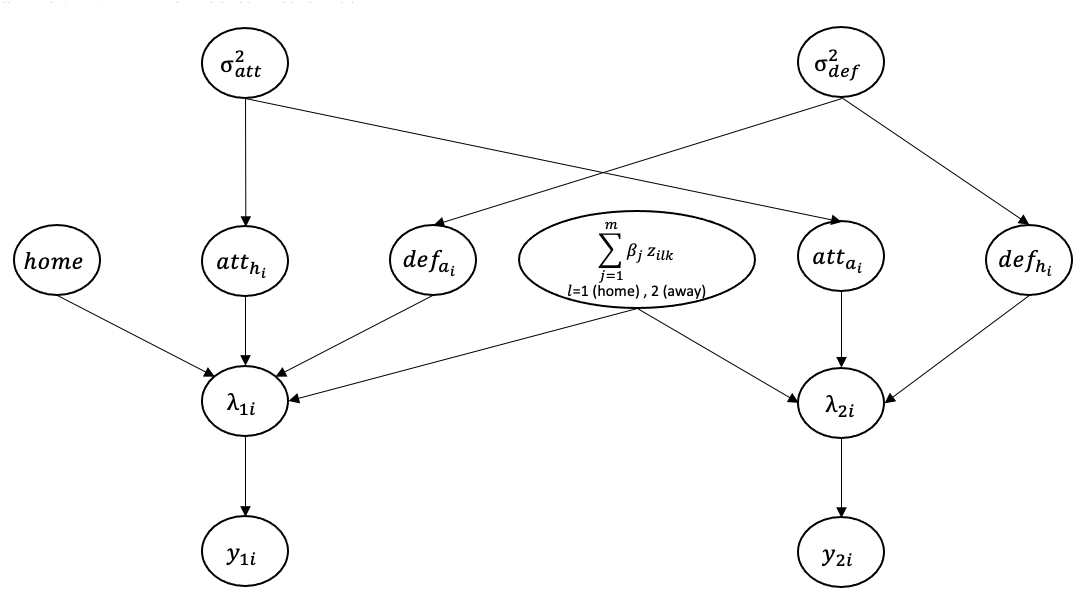
\includegraphics[width=0.7\linewidth,height=0.7\textheight]{DagDisso}

Using the formula established for the log linear model, we then fit the
model using the function\texttt{inla()} as so;

\begin{verbatim}
inla(formula = ModelFormula,
                data=LeagueData,
                family="poisson",
                control.predictor=list(compute=TRUE,link=1),
                control.compute=list(config=TRUE,dic=TRUE,waic=TRUE))`
\end{verbatim}

The \texttt{family} argument is specified asthe poisson distribution for
he response variable; number of Goals. The \texttt{data} argumnt uses
\texttt{LeagueData}, which is prepared via our created
\texttt{datprep()} function, producing a dataset of fixtures up to the
prediction round \(r\), with rounds \(1,..., r-1\) having been played
already. The intial simulation round number \texttt{r} was determined as
the next unplayed gameweek at the time of modelling, in the case of the
Premier league: \(r = 28\), La Liga: \(r = 23\), Ligue 1: \(r = 25\),
Serie A: \(r = 24\), and Bundesliga: \(r = 22\). The argument
\texttt{control.predictor} is a list specifying the predictor variables
such as \texttt{link} the link function of the model, with
\texttt{link=1} used to ensure the log link is used, and
\texttt{compute} which is a boolean variable which in this case is
\texttt{TRUE} to make sure marginal densities for the linear predictor
are also be computed. The code also specifies the
\texttt{control.compute} argument to include values in the summary for
\texttt{WAIC} and \texttt{DIC} that will be discussed further in the
model selection section.

The INlA package's methodology (Rue et al, 2009) focuses on the
posterior density of hyperparameters \(\pi( \lambda \mid y)\) and on the
conditional posterior for the latent \(\pi(x_i \mid \lambda , y_i)\) A
Laplace approximation for marginal posterior density of random effects'
hyperparamters \(\tilde{\pi}(\lambda \mid y)\) and Taylor approximation
for conditional posterior of latent
\(\tilde{\pi}(x_i \mid \lambda , y)\) From these approximations,
marginal posteriors are obtained, where integrations are carried out
numerically.
\[\tilde{\pi}(x_i \mid y_i) = \int \tilde{\pi}(\lambda \mid y)  \tilde{\pi}(x_i \mid \lambda , y)\]
Thus, using our model the predictive distribution will have a
probability mass function:

\[\tilde{\pi}(\hat{y_1} ,\hat{x_1} \mid y_1 , x_1, z_1, z_2) = \int \tilde{\pi}(\hat{y_1} ,\hat{x_1} \mid z_1 ,z_2,v)  \tilde{\pi}(v \mid y_1 , y_2,  z_1 ,z_2,)\]
Where \(\hat{y_1} ,\hat{x_1}\) are the predicted goals scored in a
future match, \(z_1\), \(z_2\) are the features used, and \(v\) is the
vector of all paramaters of the model. Then cases are considered based
on the predicted goals scored:

\begin{itemize}
\tightlist
\item
  \(\hat{y_1} > \hat{x_1} \therefore\) Home Team wins
\item
  \(\hat{y_1} < \hat{x_1} \therefore\) Away Team wins
\item
  \(\hat{y_1} = \hat{x_1} \therefore\) Draw
\end{itemize}

\pagebreak

Using values from \texttt{inla.summary.random} which outputs the INLA
model summary random effect estimates, we are able to extract the
quantiles measuring the teams' attacking and defensive strength.

Below are visual representations for the quantiles team attack and
defence effects for some of the leaguesusing only data from the 2022/23
seasons. We will discus later how this is impacted when adding more data
from previous seasons. Consider the first plot for the random effect
quantiles of Ligue 1:

\begin{center}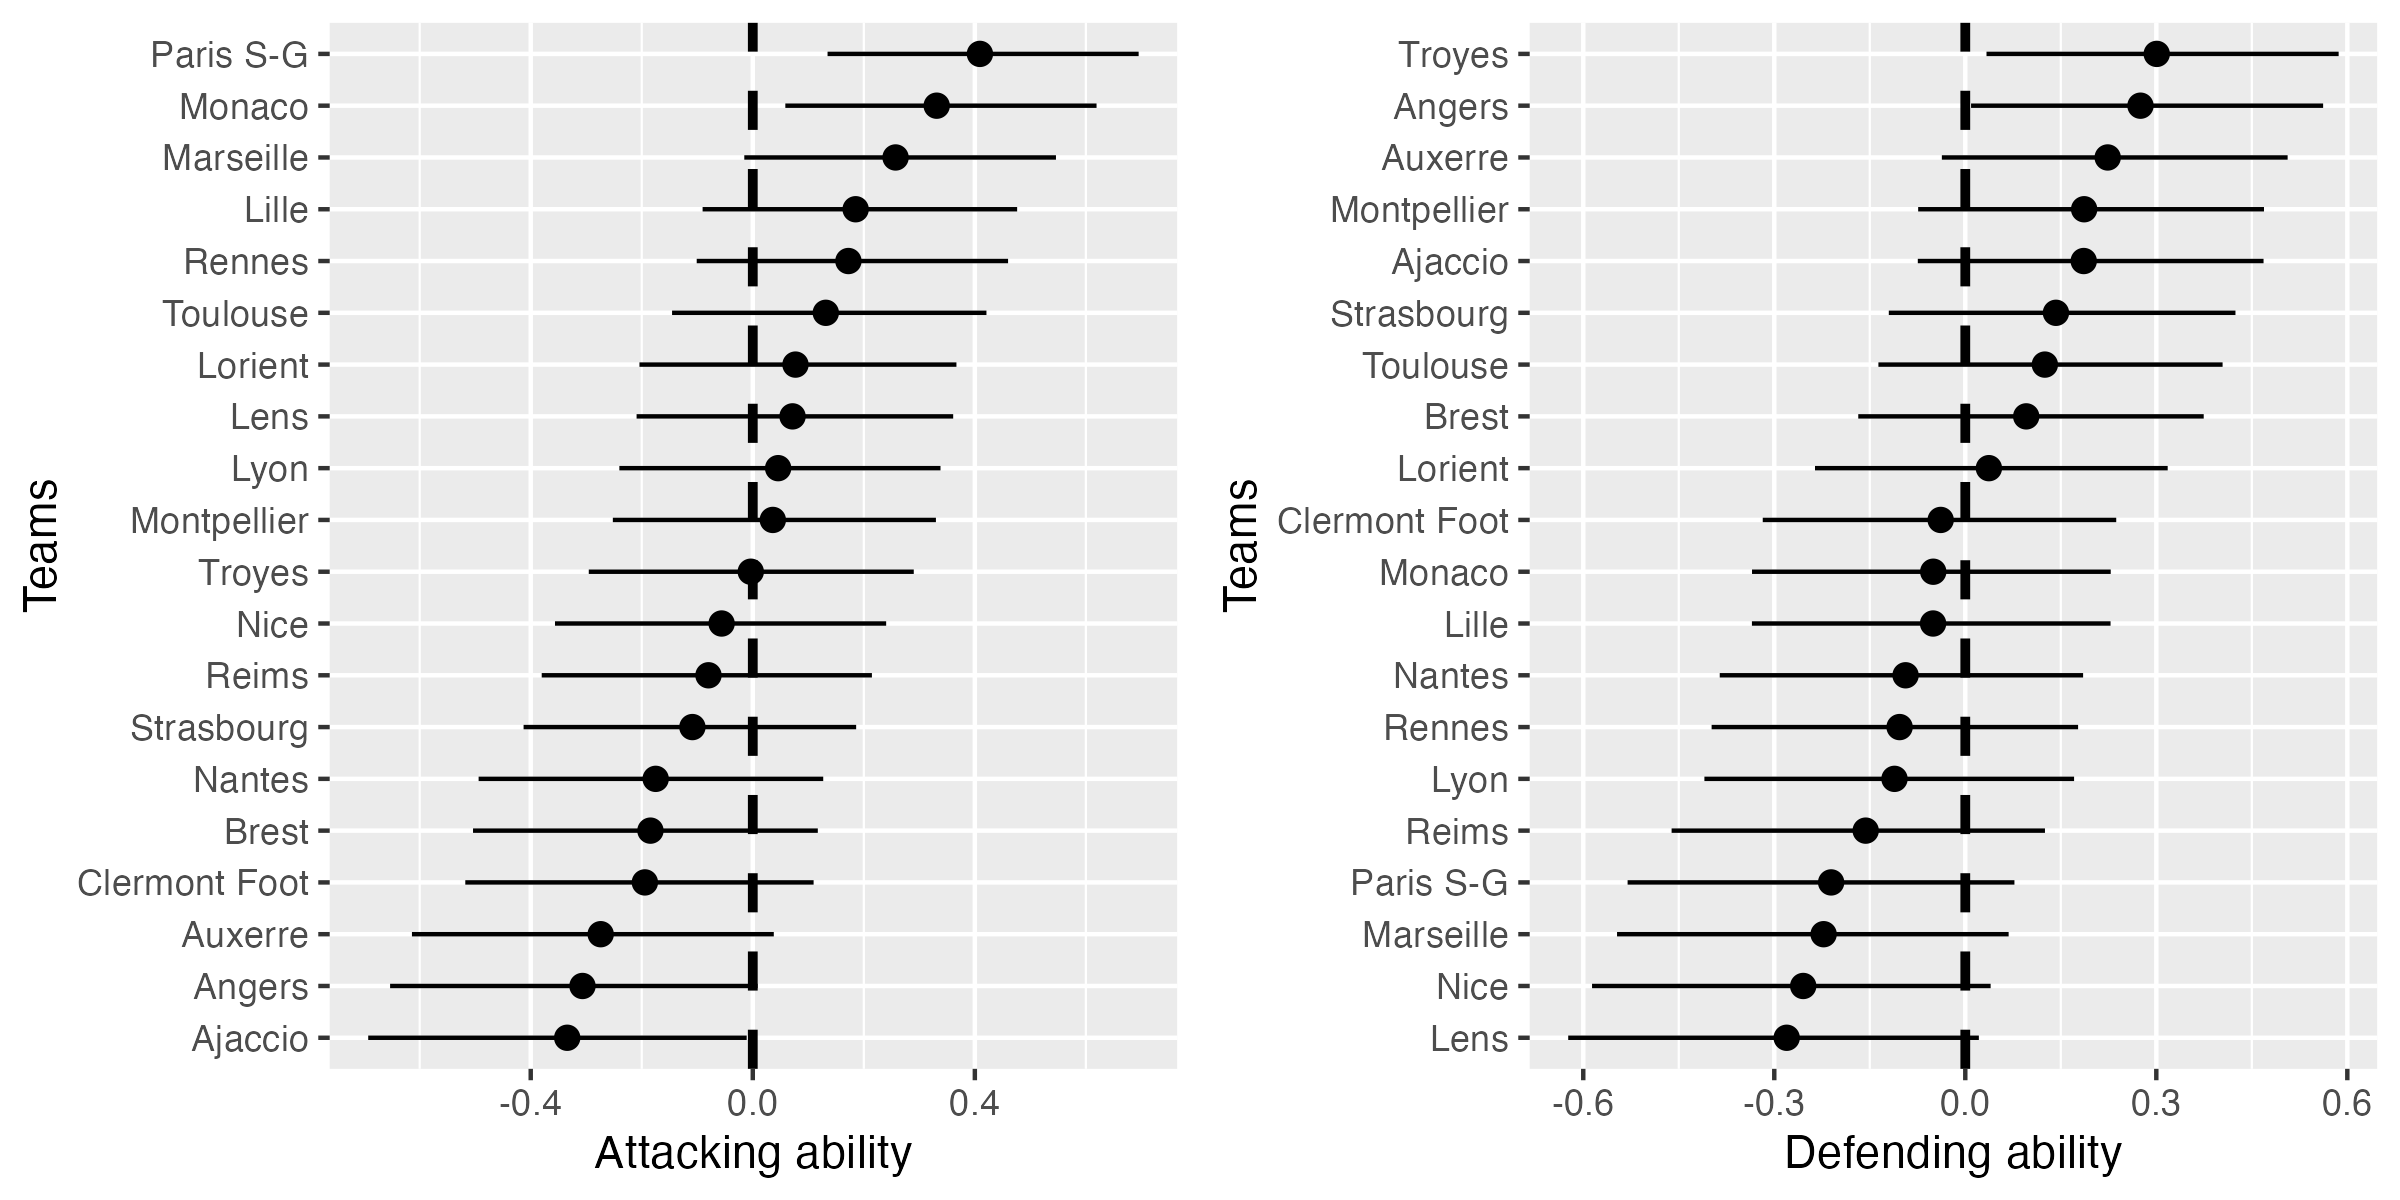
\includegraphics[width=0.7\linewidth]{l1attdef} \end{center}

For each team the range of values represent the 95\% confidence interval
for attack and defence effect estimates. The more positive values are
for the attack effect, the stronger the team's offensive capabilities,
while for the defence effect a more negative value is desirable as it
shows the team's opponents will have lower scoring propensity. PSG has
the greatest offensive capability while Ajaccio has the weakest, as for
defence Lens can be considered the best defensive team while Troyes are
the worst.

However we notice that for some leagues for example Serie A, the values
for the defence effect are considerably closer centred around the mean
0, indicating the model is not able to account for the variability in
the \texttt{Opponent} variable, due to overfitting since we only use the
2022/23 season at this stage. We discuss this later in the model
building section, and how we deal with this.

\begin{center}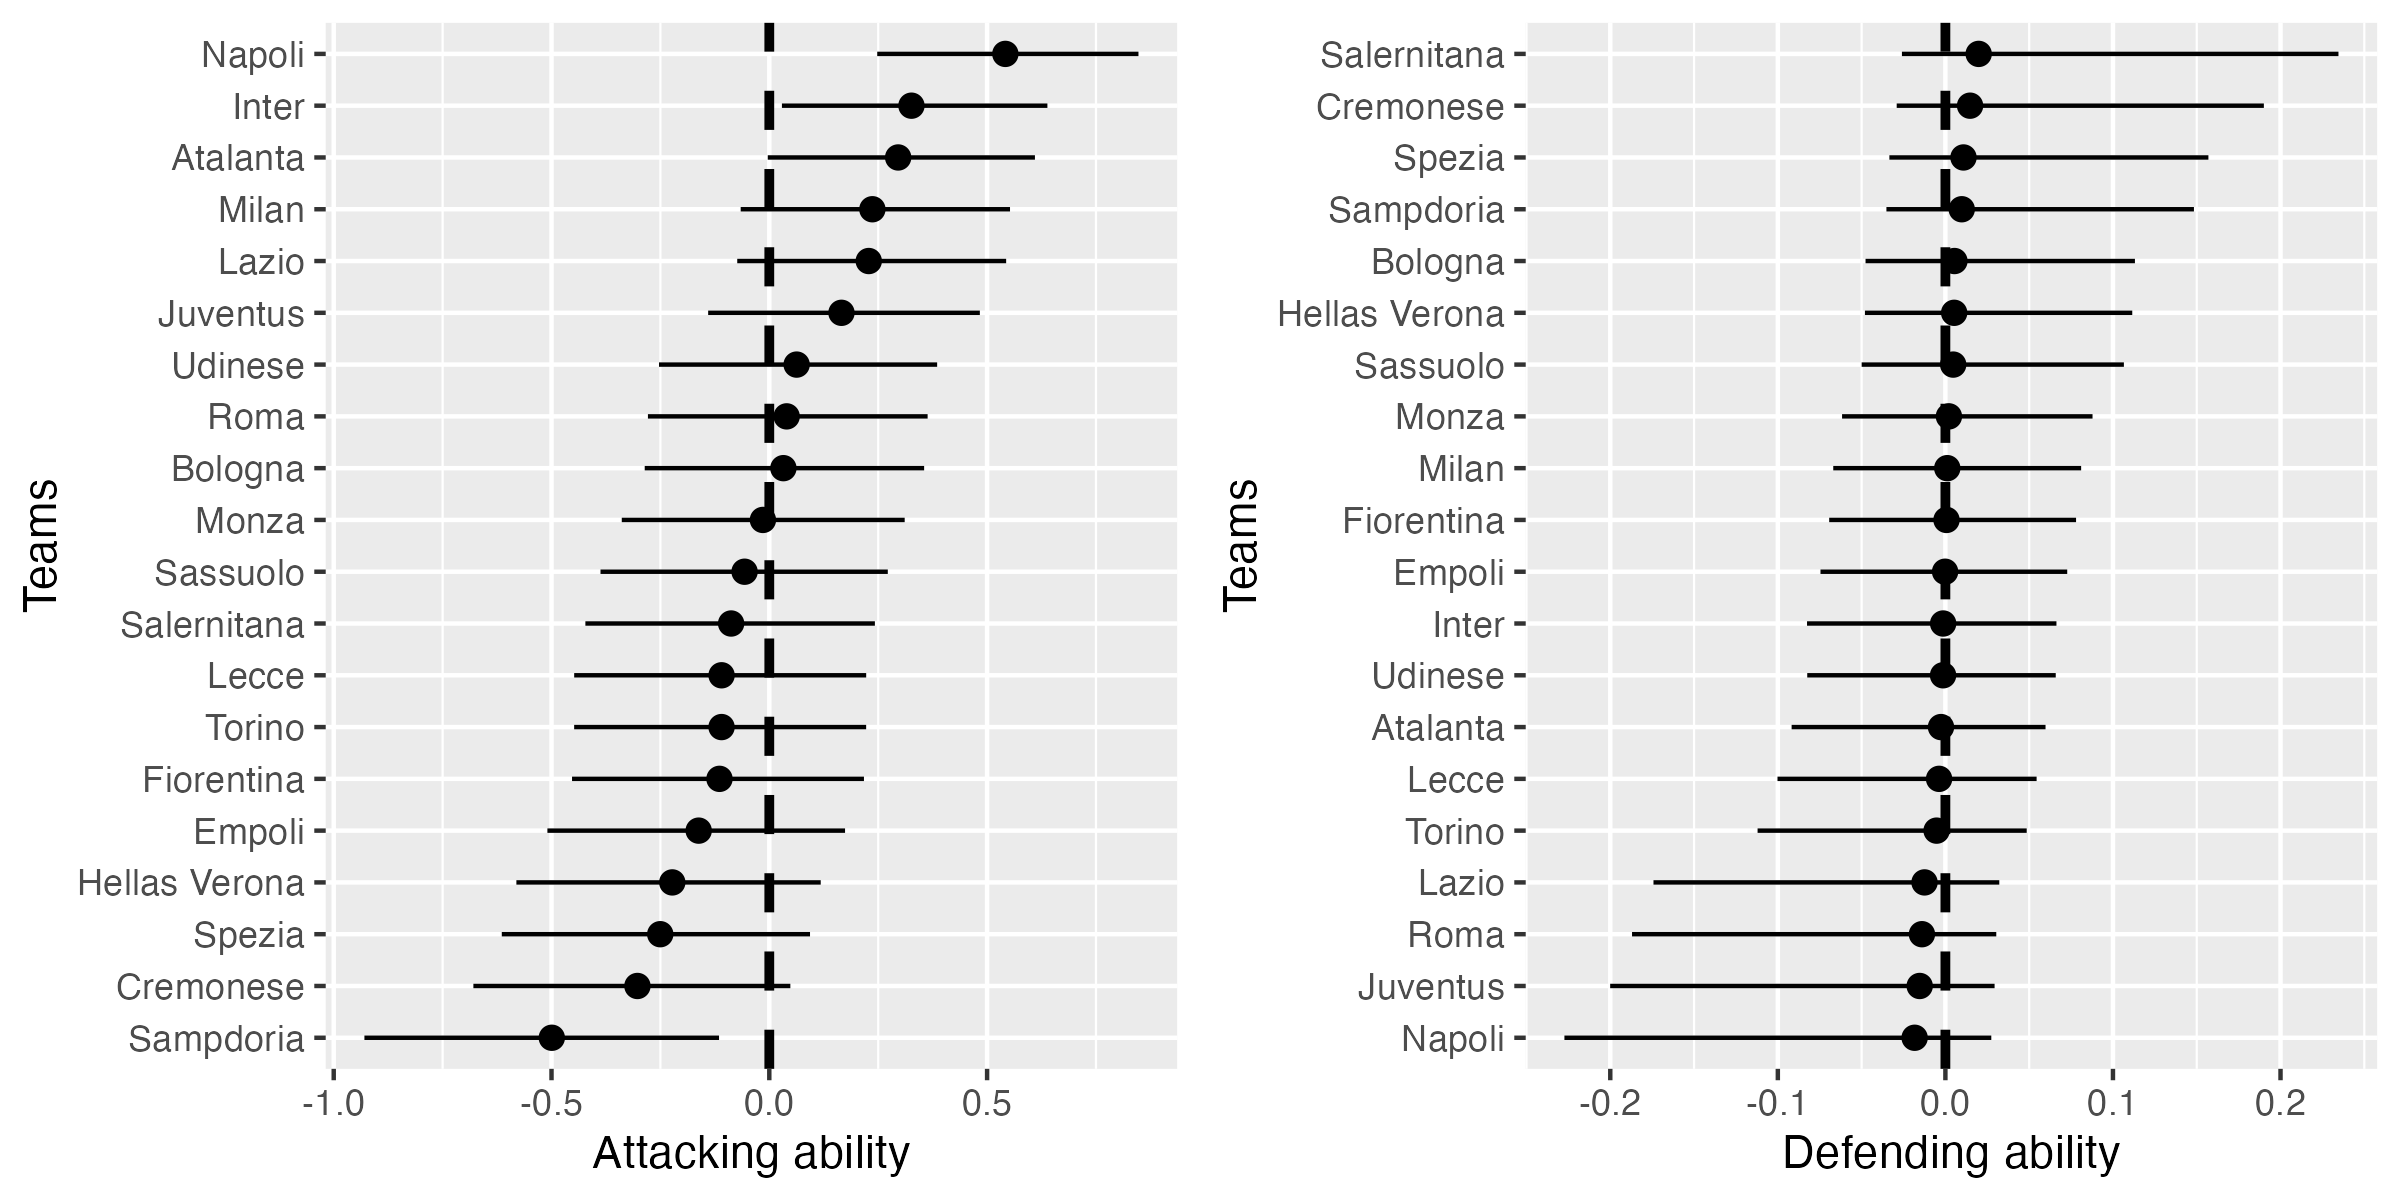
\includegraphics[width=0.7\linewidth]{saattdef} \end{center}

If we plot tttack and defence effects on the same grid, we gain an
insight of how teams proficient specific teams are at both defending and
attacking overall. Consider the case below for La Liga in the 2022/23
season showing by far how Barcelona and Real Madrid are the most
outstanding teams demonstrated by their attack effect noticeable above
the rest indicating they are more proficient at scoring goals, and
defence effects that are a lot lower than the other teams, indicating
they are not as prone to conceding goals. They are followed by a cluster
of ``next contenders''; Atletico Madrid, Real Sociedad, and Athletic
Club, leading us to suspect they would be the new ``outstanding'' clubs
should Barelona and Real Madrid leave to join the Super League. Elche
are noticeably both the worst offensive and defensive team.

\begin{figure}
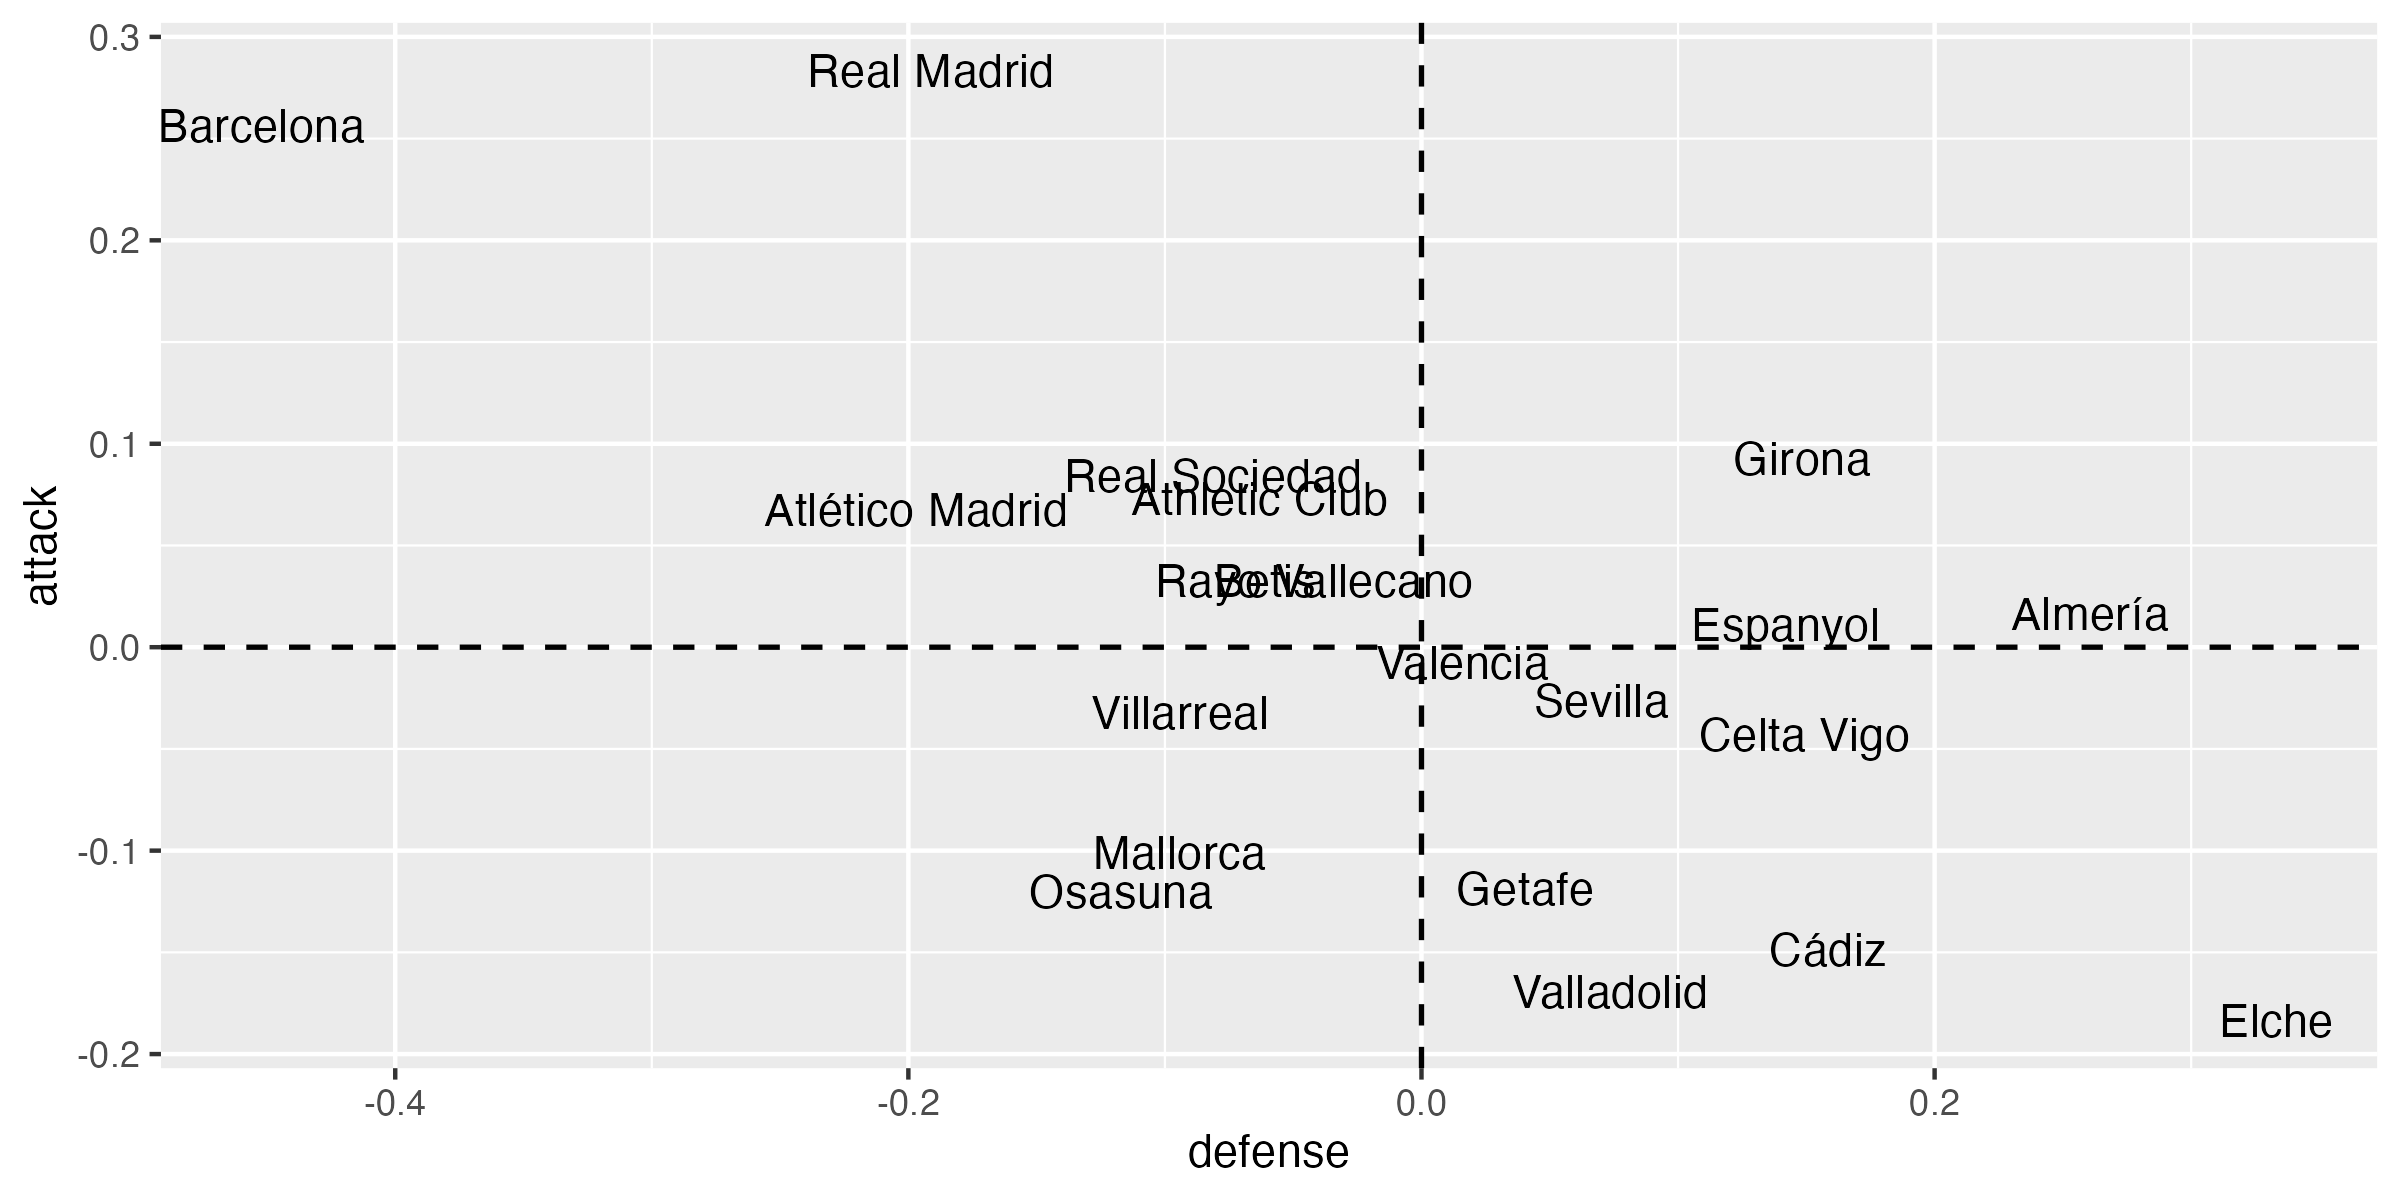
\includegraphics[width=0.9\linewidth,height=0.9\textheight]{joinedllattdef} \caption{La Liga 2022/23 Plotting Attack v Defence Effects}\label{fig:attdeflaligaexample}
\end{figure}

\hypertarget{post-processing}{%
\subsection{Post Processing}\label{post-processing}}

Having run the model through INLA, We are then able to generate the
predictions for goals scored, by simulating from the posterior
distribution for the specific round of matches. Sampling was completed
using R-INLA's method: \texttt{inla.posterior.sample}. This function
draws samples from the approximate joint posterior distribution of the
latent effects and hyperparameters which are sampled from the
configurations used to do the numerical integration. Taking the input
round number, data, model, and number of simulations (default 1000) as
inputs, we created a function \texttt{make\_scored()} that will get the
index of corresponding rows. Then the posterior samples of latent
variables are obtained using inla.posterior.sample, say
\(\hat{att_{hi}},\hat{def_{aj}}\) and \(\hat{home}\), storing the
exponentiated posterior sample values. Then we compute the predicted
scoring intensity paramter by each team in the specific round:

\[\hat{\lambda_{ij}} = \exp(\hat{att_{hi}} + \hat{def_{aj}} + \hat{home} + \text{offset})\]
Finally the function generates the predictions for the number of goals
by simulating from a Poisson Distribution using \texttt{rpois()}, with
the predicted scoring intensity parameter:

\[goals_{ij} \sim  \text{Poisson} ( \hat{\lambda_{ij}} )\]

\hypertarget{programmed-functions-in-r}{%
\subsubsection{Programmed Functions in
R}\label{programmed-functions-in-r}}

The code used in the model building process includes utility functions
that manipulate, visualise, and simulate from our dataset to generate
predictions.

\hypertarget{prediction-processing-functions}{%
\paragraph{Prediction Processing
Functions}\label{prediction-processing-functions}}

\begin{itemize}
\item
  \texttt{datprep()} , preps the data of a league to be used in our
  \texttt{runINLA()} function.
\item
  \texttt{runINLA()} , runs the INLA model after specifying the formula,
  data for given round, posterior family,
\item
  \texttt{make\_scored()} , Processing function create to predict the
  number of goals scored by a team in a given fixture round.
\end{itemize}

\hypertarget{visulisation-functions}{%
\paragraph{Visulisation Functions:}\label{visulisation-functions}}

\begin{itemize}
\item
  \texttt{team\_strength()} , Display Only Attack or Defence Defence
  random effects for teams in a league
\item
  \texttt{attack\_defense()} , Display Both Attack and Defence effects
  on the same plot, from the INLA model summary
\item
  \texttt{outcome\_predict()} , gives the predicted probabilities of
  either winning, losing, or drawing a match.
\item
  \texttt{joint\_marginal()} , gives the plot of the joint posterior
  probabilities for specified teams Plots the joint posterior
  distributions of all the possible scores between two team given the
  predicted goals from \texttt{make\_scored()}
\end{itemize}

\hypertarget{post-processing-functions}{%
\paragraph{Post-Processing Functions}\label{post-processing-functions}}

\begin{itemize}
\item
  \texttt{updated\_unplayed()} , extracts the unplayed fixtures for a
  given round and inputs the most common result ( i think this should
  instead be inputting just the sample mean of the column of goals
  scored for the team rounded?)
\item
  \texttt{update\_footie()} , updates the premfootie dataset with the
  goal predictions
\item
  \texttt{var\_updater()} , updates the other variables in the dataset
  as a result of the goal predictions
\item
  \texttt{roundNinla()} , streamlines the simulating process, by
  completing all of the above 3 post-processing for a given round N ,
  e.g round 24
\end{itemize}

\hypertarget{outcome-predictions}{%
\subsection{Outcome predictions}\label{outcome-predictions}}

Running \texttt{inla.summary} we are able to extract coefficients for
fixed and random effect estimates of our models. For example in the case
below we consider a full model with all covariates to examine results in
the 2022/23 Serie A season:

\begin{table}

\caption{\label{tab:exampleseriesummaryoutput}Serie A Fixed Effects; only 2022-2023 Seasons}
\centering
\begin{tabular}[t]{l|r}
\hline
  & mean\\
\hline
(Intercept) & -0.739\\
\hline
Home & -0.014\\
\hline
diff\_point & 0.001\\
\hline
diff\_rank & 0.004\\
\hline
form & 0.123\\
\hline
rel\_strength & 0.303\\
\hline
days\_since\_last & 0.000\\
\hline
Gpg & 0.163\\
\hline
GCpg & 0.284\\
\hline
GDdiff & 0.179\\
\hline
\end{tabular}
\end{table}

\begin{table}

\caption{\label{tab:exampleseriesummaryoutput}Serie A Hyperparameters and Precision; only 2022-2023 Seasons}
\centering
\begin{tabular}[t]{l|r}
\hline
  & mean\\
\hline
Precision for factor(Team) & 19027.68\\
\hline
Precision for factor(Opponent) & 19118.21\\
\hline
\end{tabular}
\end{table}

From the model summary's fixed effect table, we see that a few variables
namely Rank Difference, Point Difference, and Days Since Last Game, have
negligable coefficient means relative to the other variables. We also
notice from the output of the model hyperparameter summary that the
precision for the random effects are significantly high, indicating very
little variation is accounted for both random effects effects.\\
Both output summaries indicate that the use of some variables, along
with the use of only ony season's worth of data may result in the model
overfitting the data, leading us to the next section where we aim to
mitigate this.

\hypertarget{introduction-of-multiple-seasons-data}{%
\subsection{Introduction of Multiple Seasons'
Data}\label{introduction-of-multiple-seasons-data}}

As aforementioned in `The Model' section, upon plotting the defence
effect for leagues such as Serie A, we saw effect estimates that were
too closely centred around the mean, and the precision for the
hyperparameters were suspiciously higher than one would expect. This
highlighted the lack of variability accounted for in the model due to
overfitting Thus the model may be capturing the noise rather than the
underlying pattern, in this case resulting in the lack of variability in
th Opponent random effect.

To mitigate this concern we include the use of multiple seasons data as
opposed to using a single season, that only provides 760 rows of data.
With the inclusion of the 2019/20, 2020/21, and 2021/22 along with the
2022/23 seasons, this now results in dataframes with 3040 rows of data
for each league. The effects of overfitting are also demonstrated in the
random effect quantile plots, particularly for the Opponent (Defence)
factor. Consider the case of the Premier League, where the magnitude of
the effects are considerably small and closely centred around the mean;

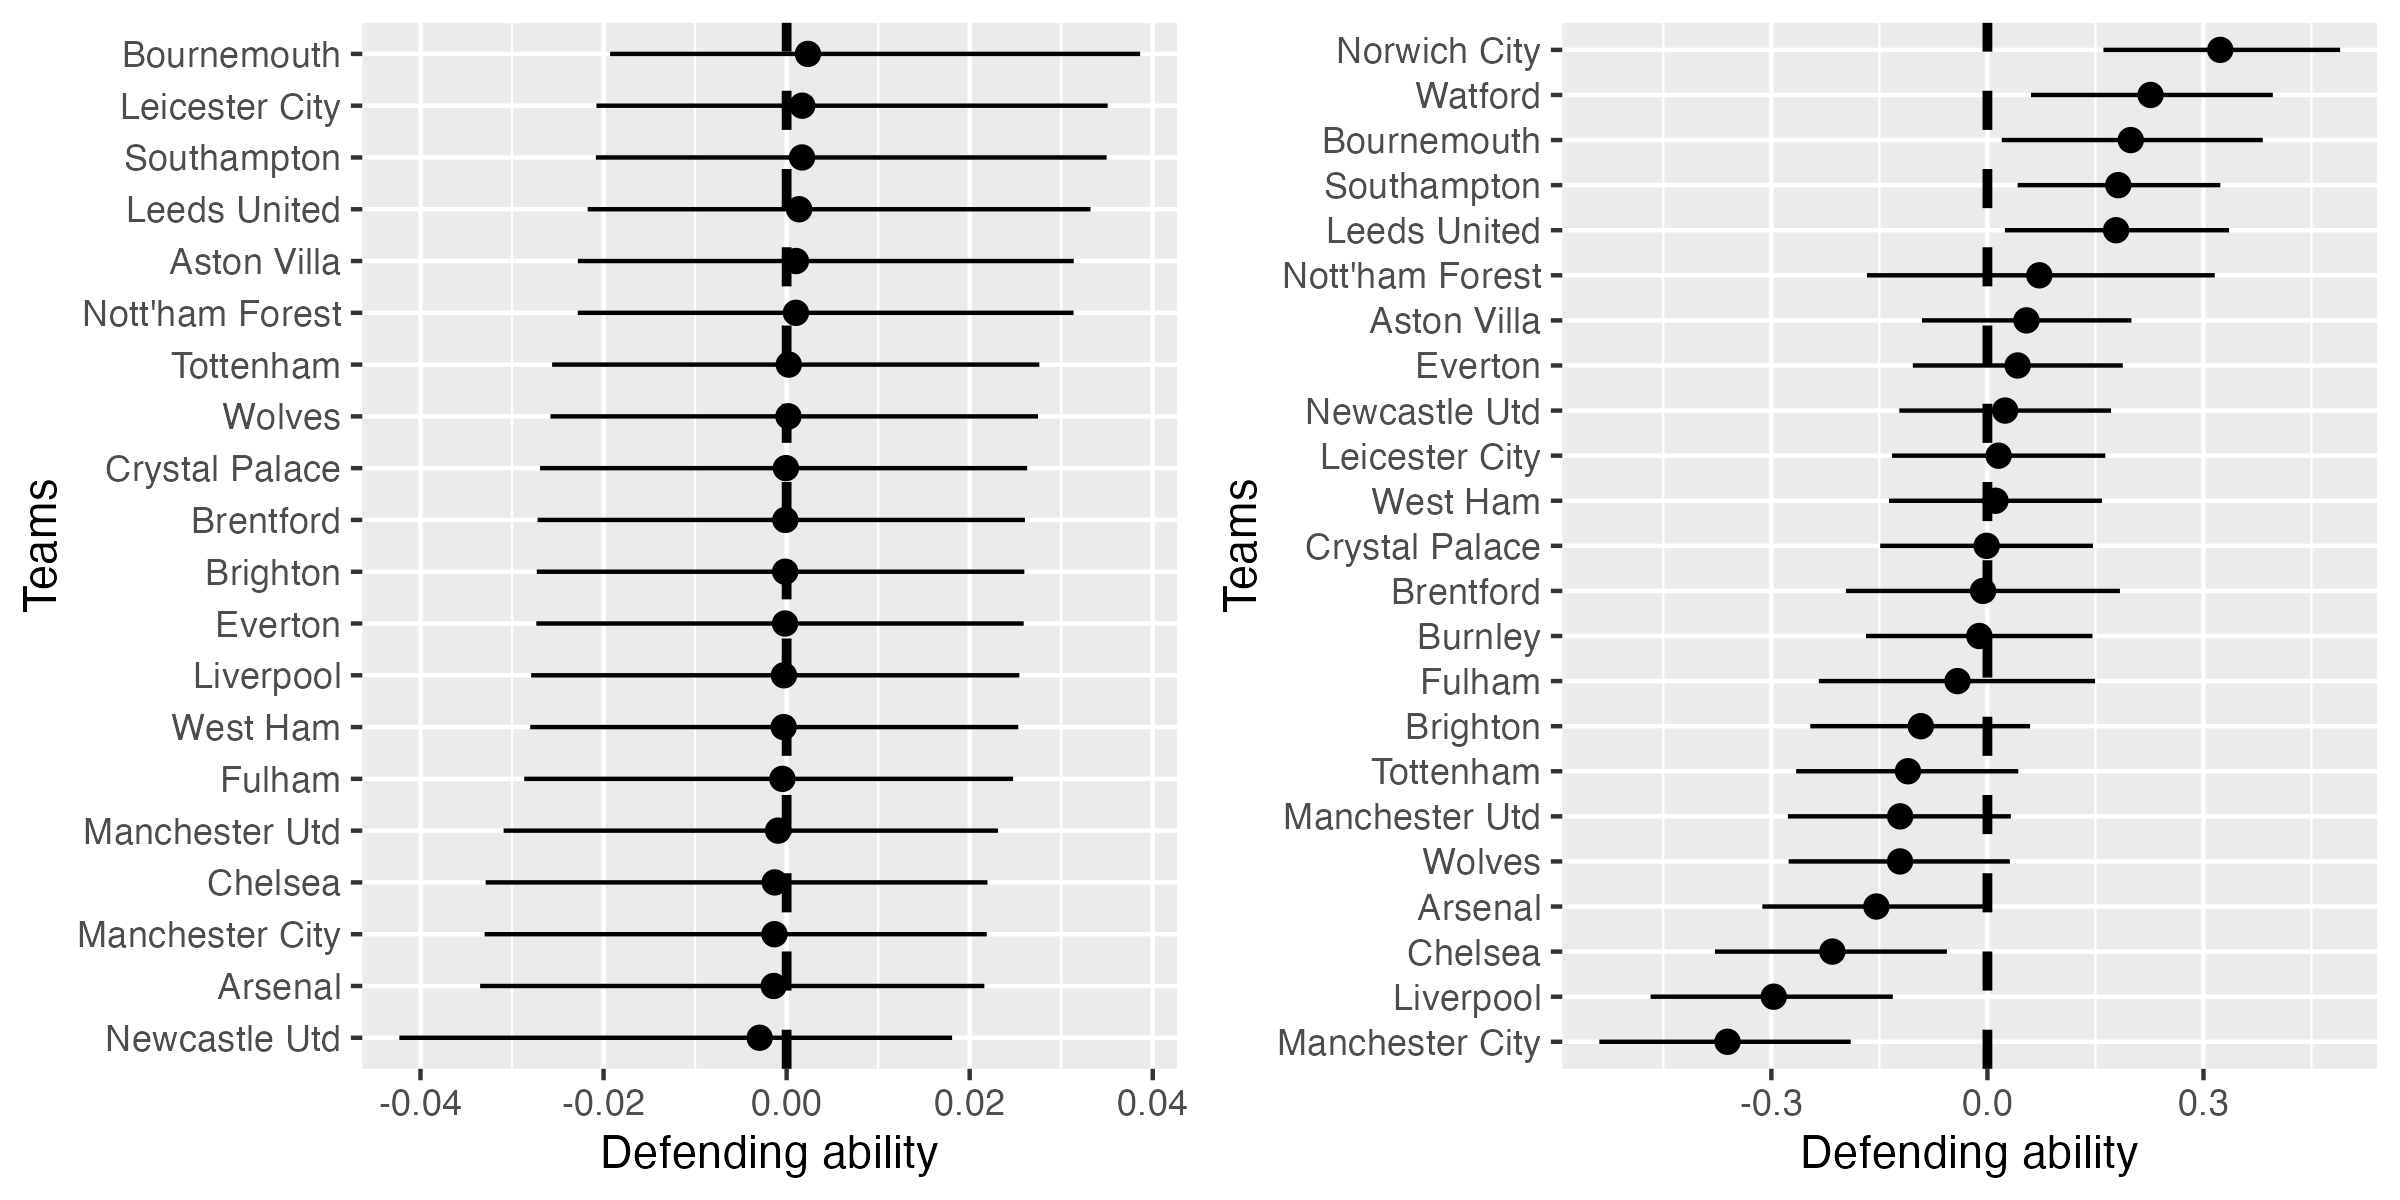
\includegraphics[width=0.9\linewidth,height=0.9\textheight]{allvssingledefprem}

After adding multiple seasons of data, we see how there is now
noticeable variability in the defence effect for all teams. Thus
demonstrated how we have mitigated the impact of overfitting by adding
more data from multiple seasons. We also see this in the inla.summary
output shown below, where the precision for the model hyperparameters
are considerably smaller; mean 18194.995 when only using 2022/23
compared to 33.254 for 2019-2023 data.

\begin{table}

\caption{\label{tab:premallsinglesumcomp}Hyperparameter Precision using only 2022-2023 Season}
\centering
\begin{tabular}[t]{l|r}
\hline
  & mean\\
\hline
Precision for factor(Team) & 11.605\\
\hline
Precision for factor(Opponent) & 18194.995\\
\hline
\end{tabular}
\end{table}

\begin{table}

\caption{\label{tab:premallsinglesumcomp}Hyperparameter Precision using 2019-2023 Seasons}
\centering
\begin{tabular}[t]{l|r}
\hline
  & mean\\
\hline
Precision for factor(Team) & 12.364\\
\hline
Precision for factor(Opponent) & 33.254\\
\hline
\end{tabular}
\end{table}

\hypertarget{result-generation}{%
\subsection{Result Generation}\label{result-generation}}

Now that we are able to generate predictions using the
\texttt{inla.posterior.sample} method for the number of goals scored for
each team after a given round, we are then able to get predicted match
outcomes for the selected fixtures. In similar research the use of
posterior means or medians is used from both individual team's marginal
distribution, however in our modelling we use the most probable outcome
from the joint posterior predictive distribution in each fixture,
i.e.~the most common row outcome between two teams after each n row
simulations are complete.

For instance, using the baseline model in round 23 of the 2022/23 La
Liga season, in a match between Villarrael and Getafe. We can visually
display the joint marginal distribution of goals scored in this specific
match, using our created function \texttt{joint\_marginal()}.

\begin{figure}
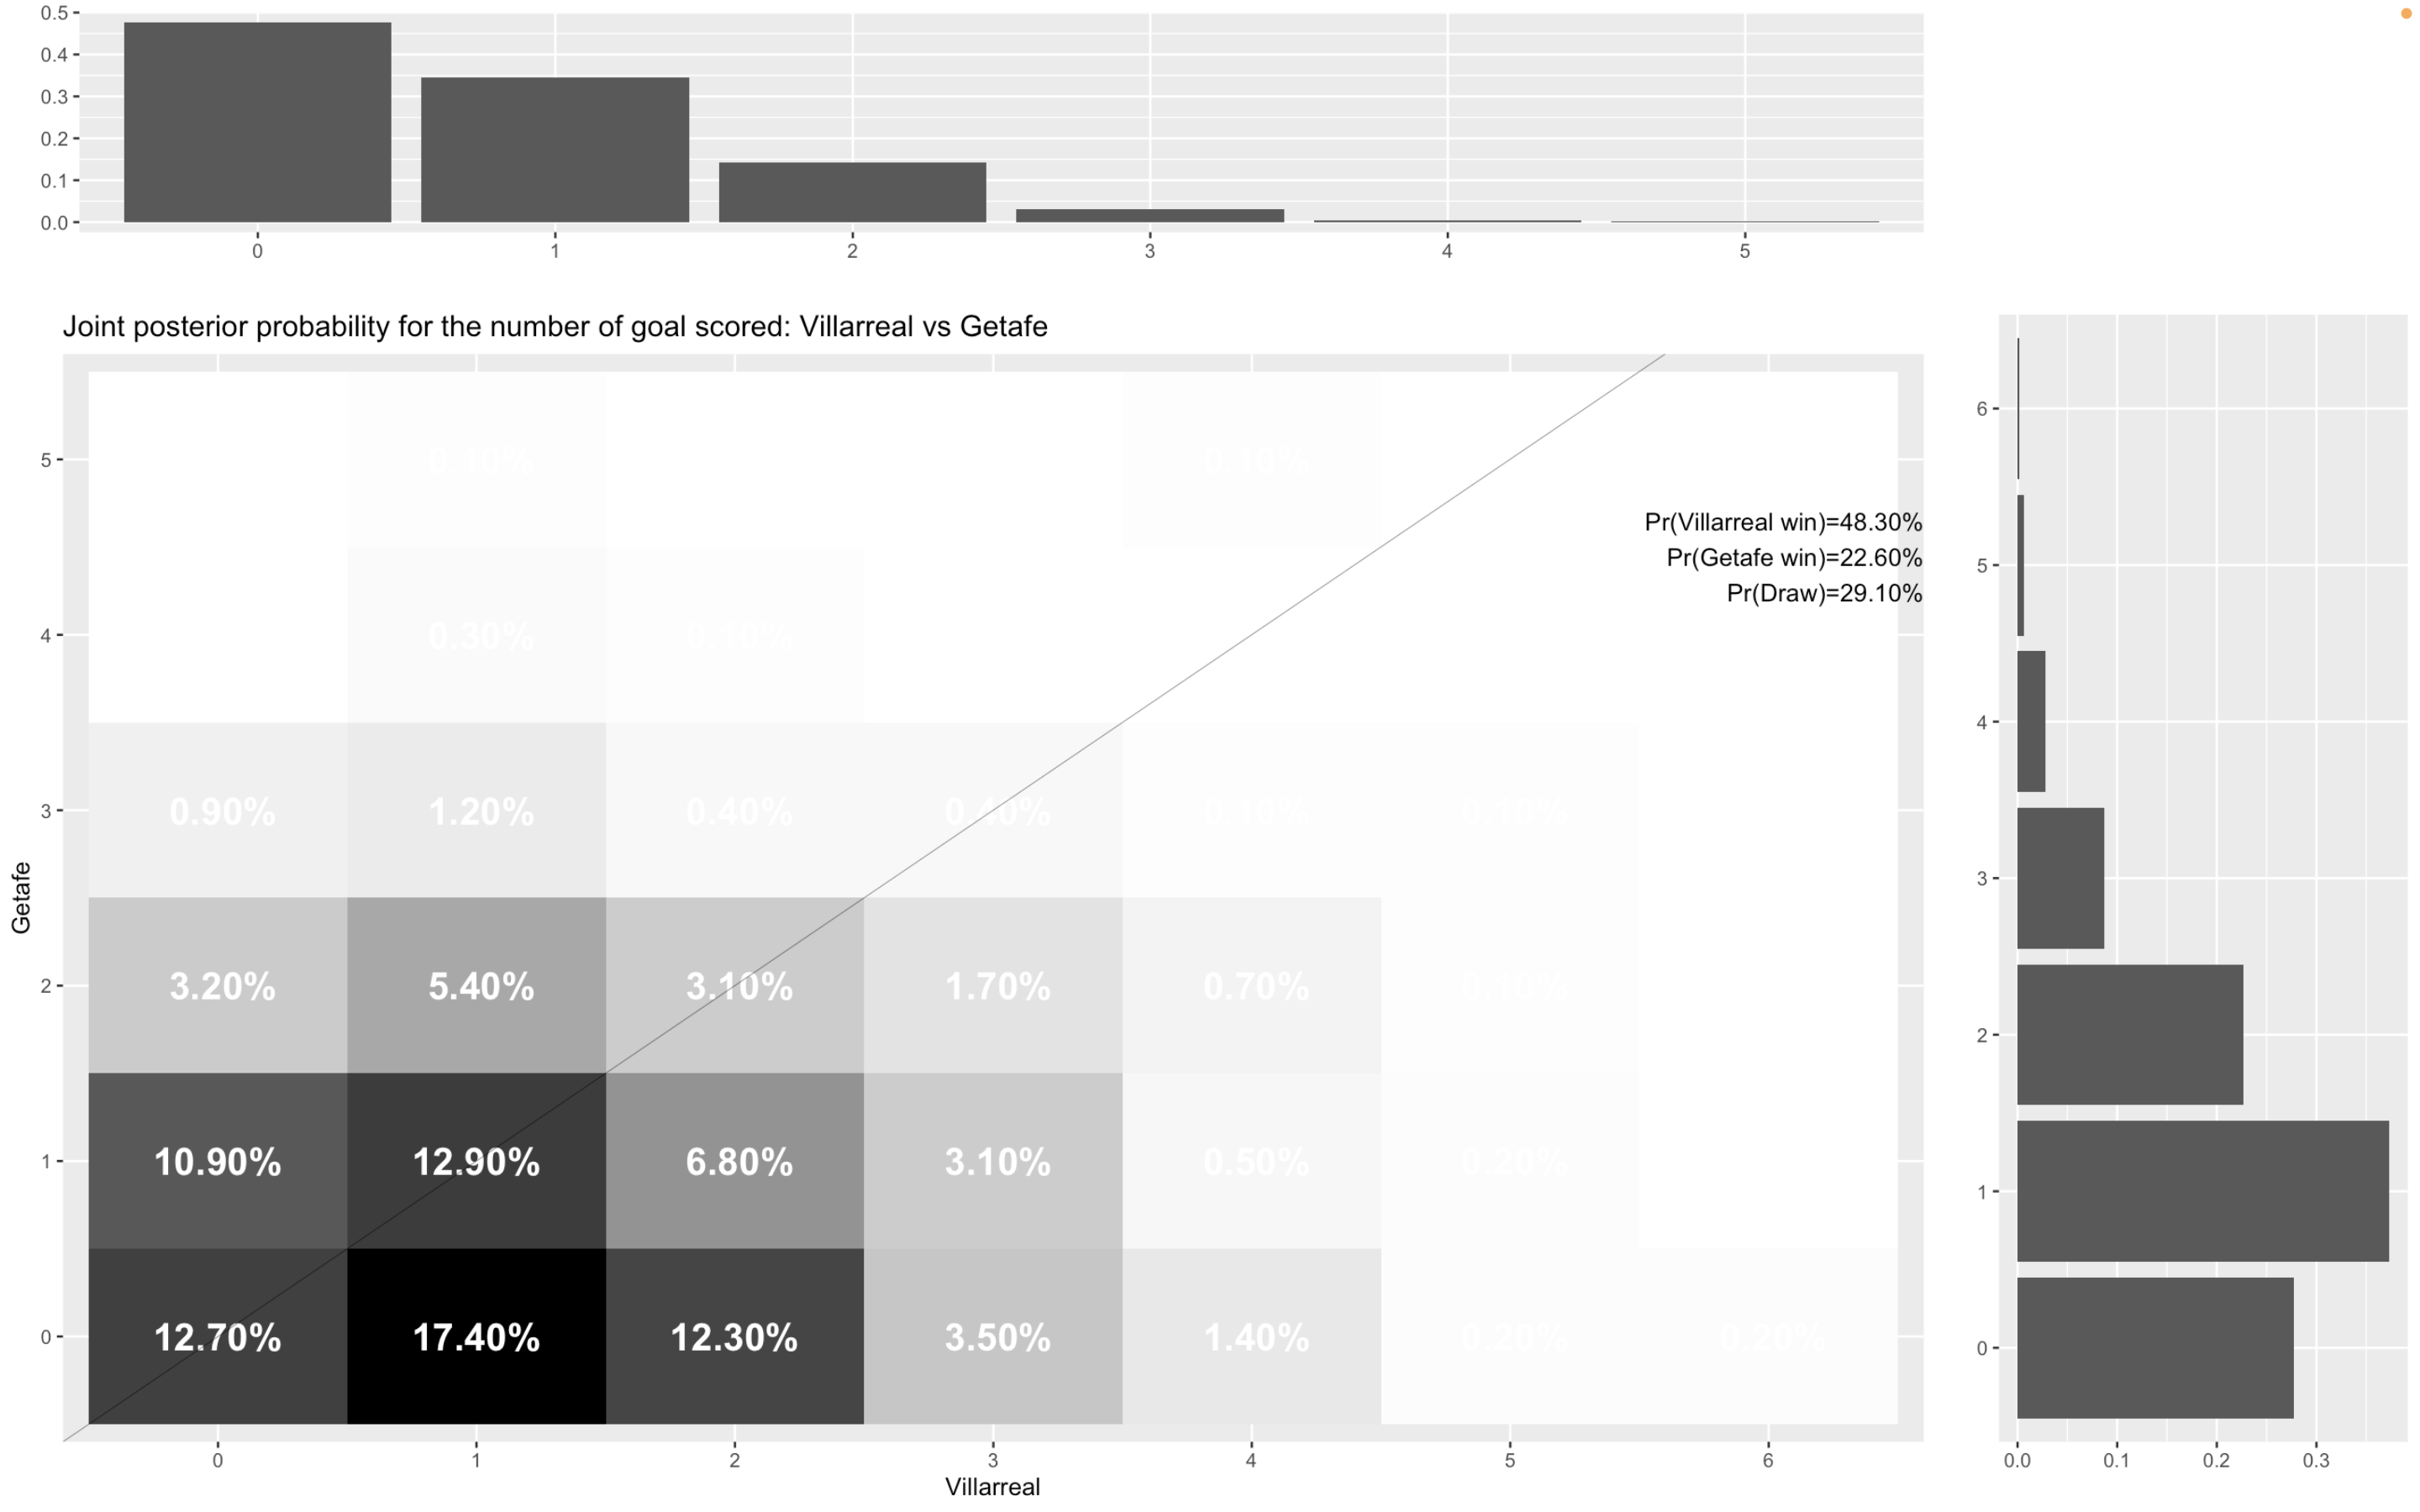
\includegraphics[width=0.9\linewidth,height=0.9\textheight]{getafevillarrael} \caption{Plotting the Joint Marginal Distriubtion of goals scored between Villarrael and Getafe}\label{fig:unnamed-chunk-1}
\end{figure}

Here the percentages represent the proportion of outcomes with the given
result, thus in this case 17.4\% of outcomes in the match see Villarrael
as victors specifically with a score of 1-0.

We see the probability of every possible outcome from the joint
posterior distribution, along with the overall probability of winning,
drawing, or losing found using our created \texttt{outcome\_predict()}
function. The histograms represents the sampled marginal posterior
distribution for teams individually, with highest density of 0 goal
scored for Getafe (top), and 1 for Villarrael (Right).

After determining the most likely result of relevant `Goal' column, as
well as the associated variables derived from it such as Points , Goal
Difference, Relative Strength etc. Although as before these are not used
in the baseline model.

In the case of Bundesliga, we calculate the cumulative points determined
from goals scored in each game, and derive the league table at the end
of the season: We first show the results when using the Mean of each
teams predicted goals after n simulations, compared to using the joint
predictive posterior distribution. Using means shows Bayern Munich
winning the league, where as the most probable outcome from the joint
distributions leads to Dortmund winning the league

\hypertarget{model-selection}{%
\subsection{Model Selection:}\label{model-selection}}

Typically in INLA and hierarchical modelling (Rue et al.~2009), the use
of Deviance Information Criterion and
Watanabe-Alike-Information-Criterion are use as methods of comparing
models in context. DIC is a model that is analogous to the Akaike
information criterion (AIC) used in estimating prediction error, instead
measuring the trade off between model fit and complexity calculated as
follows: \[ DIC(\lambda) =  D(\bar{\lambda}) + 2p_D \] where
\(D(\bar{\lambda})\) is the deviance at the posterior mean of the
parameters and \(p_D\) is the effective number of parameters.

Similarly the Watanabe-Akaike Information Criterion is a indicator of
singular model performance. As defined by Watanabe himself, (Gelman et
al.~2014) WAIC is the ``negative of the average log pointwise predictive
density and thus is divided by n, and does not have the factor of 2'',
although in INLA is is scaled by factor of 2 for comparability with DIC
and other measures of deviance. DIC makes the assumption that the
posterior is approximately multivariate normal, while WAI can be
numerically calculated without information on the true distribution.
WAIC also an extension of the widely used AIC in the Bayesian context,
and also offers the bonus of no need for effective parameters, again
unlike DIC. Given the added applicability to general BHM methods, the
WAIC is a better indicator of model suitability.

\hypertarget{optimised-model-formulas-for-log-linear-models}{%
\subsection{Optimised Model Formulas for Log Linear
Models}\label{optimised-model-formulas-for-log-linear-models}}

\hypertarget{premier-league}{%
\subsubsection{Premier League}\label{premier-league}}

Below is a table showing the top 10 models with the lowest WAIC,
indicating top 10 most suitable models given the fact that lower WAIC
demonstrates desirable lower deviance. Consider the example below of the
Premier League, where the formula that results in the lowest WAIC
includes added covariates Form, Goals Per Game (Gpc), Goals Conceded Per
Game (GCpg), and Goal Difference-Difference between teams (GDdiff).

\begin{table}[!h]

\caption{\label{tab:unnamed-chunk-2}Top 10 Model Combinations By WAIC: Premier League}
\centering
\begin{tabular}[t]{c|c}
\hline
Formula & WAIC\\
\hline
Goal \textasciitilde{} Home + form + Gpg + GCpg + GDdiff + Att + Def & 6642.466\\
\hline
Goal \textasciitilde{} Home + form + days\_since\_last + Gpg + GCpg + GDdiff + Att + Def & 6643.580\\
\hline
Goal \textasciitilde{} Home + rel\_strength + form + Gpg + GCpg + GDdiff + Att + Def & 6643.728\\
\hline
Goal \textasciitilde{} Home + diff\_rank + form + Gpg + GCpg + GDdiff + Att + Def & 6643.918\\
\hline
Goal \textasciitilde{} Home + Gpg + GCpg + GDdiff + Att + Def & 6644.575\\
\hline
Goal \textasciitilde{} Home + rel\_strength + form + days\_since\_last + Gpg + GCpg + GDdiff + Att + Def & 6644.813\\
\hline
Goal \textasciitilde{} Home + rel\_strength + diff\_rank + form + Gpg + GCpg + GDdiff + Att + Def & 6644.870\\
\hline
Goal \textasciitilde{} Home + diff\_rank + form + days\_since\_last + Gpg + GCpg + GDdiff + Att + Def & 6645.032\\
\hline
Goal \textasciitilde{} Home + days\_since\_last + Gpg + GCpg + GDdiff + Att + Def & 6645.622\\
\hline
Goal \textasciitilde{} Home + rel\_strength + Gpg + GCpg + GDdiff + Att + Def & 6645.838\\
\hline
\end{tabular}
\end{table}

Thus the optimal formula for the Premier League model after this part of
the model building process is of the form:

Home Goals in game i:
\[log(\lambda_{1i}) =  att_{h_i} + def_{a_i} + \beta_1 Home_j + \beta_2 form + \beta_3 Gpg + \beta_4 GCpg +  \beta_5GDdiff\]
Away Goals in game i:

\[log(\lambda_{2i}) = att_{h_i} + def_{a_i} + \beta_1 form + \beta_2 Gpg + \beta_3 GCpg +  \beta_4 GDdiff\]

As for the other domestic leagues, the optimised formulae for the log
linear models are:

\hypertarget{la-liga}{%
\subsubsection{La Liga:}\label{la-liga}}

Home Team:
\[log(\lambda_{1i}) =   att_{a_i} + def_{h_i} +  \beta_1 Home + \beta_2 Gpg + \beta_3 GCpg + \beta_4 GDdiff\]
Away Team:
\[log(\lambda_{2i}) =   att_{h_i} + def_{a_i} + \beta_1 Gpg + \beta_2 GCpg +  \beta_3 GDdiff\]

\hypertarget{serie-a}{%
\subsubsection{Serie A:}\label{serie-a}}

Home Team:
\[log(\lambda_{1i}) =   att_{a_i} + def_{h_i} +  \beta_1 Home + \beta_2 Gpg + \beta_3 GCpg + \beta_4 GDdiff + \beta_5 Form\]
Away Team:
\[log(\lambda_{2i}) =   att_{h_i} + def_{a_i} + \beta_1 Gpg + \beta_2 GCpg +  \beta_3 GDdiff + \beta_4 form\]

\hypertarget{bundesliga}{%
\subsubsection{Bundesliga:}\label{bundesliga}}

Home Team:
\[log(\lambda_{1i}) =   att_{a_i} + def_{h_i} +  \beta_1 Home + \beta_2 Gpg + \beta_3 GCpg + \beta_4 GDdiff\]
Away Team:
\[log(\lambda_{2i}) =   att_{h_i} + def_{a_i} + \beta_1 Gpg + \beta_2 GCpg +  \beta_3 GDdiff\]

\hypertarget{ligue-1}{%
\subsubsection{Ligue 1:}\label{ligue-1}}

Home Team:
\[log(\lambda_{1i}) =   att_{a_i} + def_{h_i} +  \beta_1 Home + \beta_2 Gpg + \beta_3 GCpg + \beta_4 GDdiff + \beta_5 diffrank\]
Away Team:
\[log(\lambda_{2i}) =   att_{h_i} + def_{a_i} + \beta_1 Gpg + \beta_2 GCpg +  \beta_3 GDdiff + \beta_4 diffrank\]
\#\# Aditional Covariate Consideration

We also explore the addition of other covariates that may further
improve model performance. First, a time component that aims to address
team's difference in performance over time. This is added to the INLA
model using
\texttt{f(id\_date,model="rw2",replicate=as.numeric(factor(Team)))}. A
Random Walk model of order 2 \texttt{model="rw2"} based on the fixture
date variable representing the time component, is computed separately
for each team \texttt{replicate=as.numeric(factor(Team))}. The effects
from the Random Walk over the course of the dates in our dataset
(between the start of the 2019 season and end of the 2023 season) are
shown in the plot below:

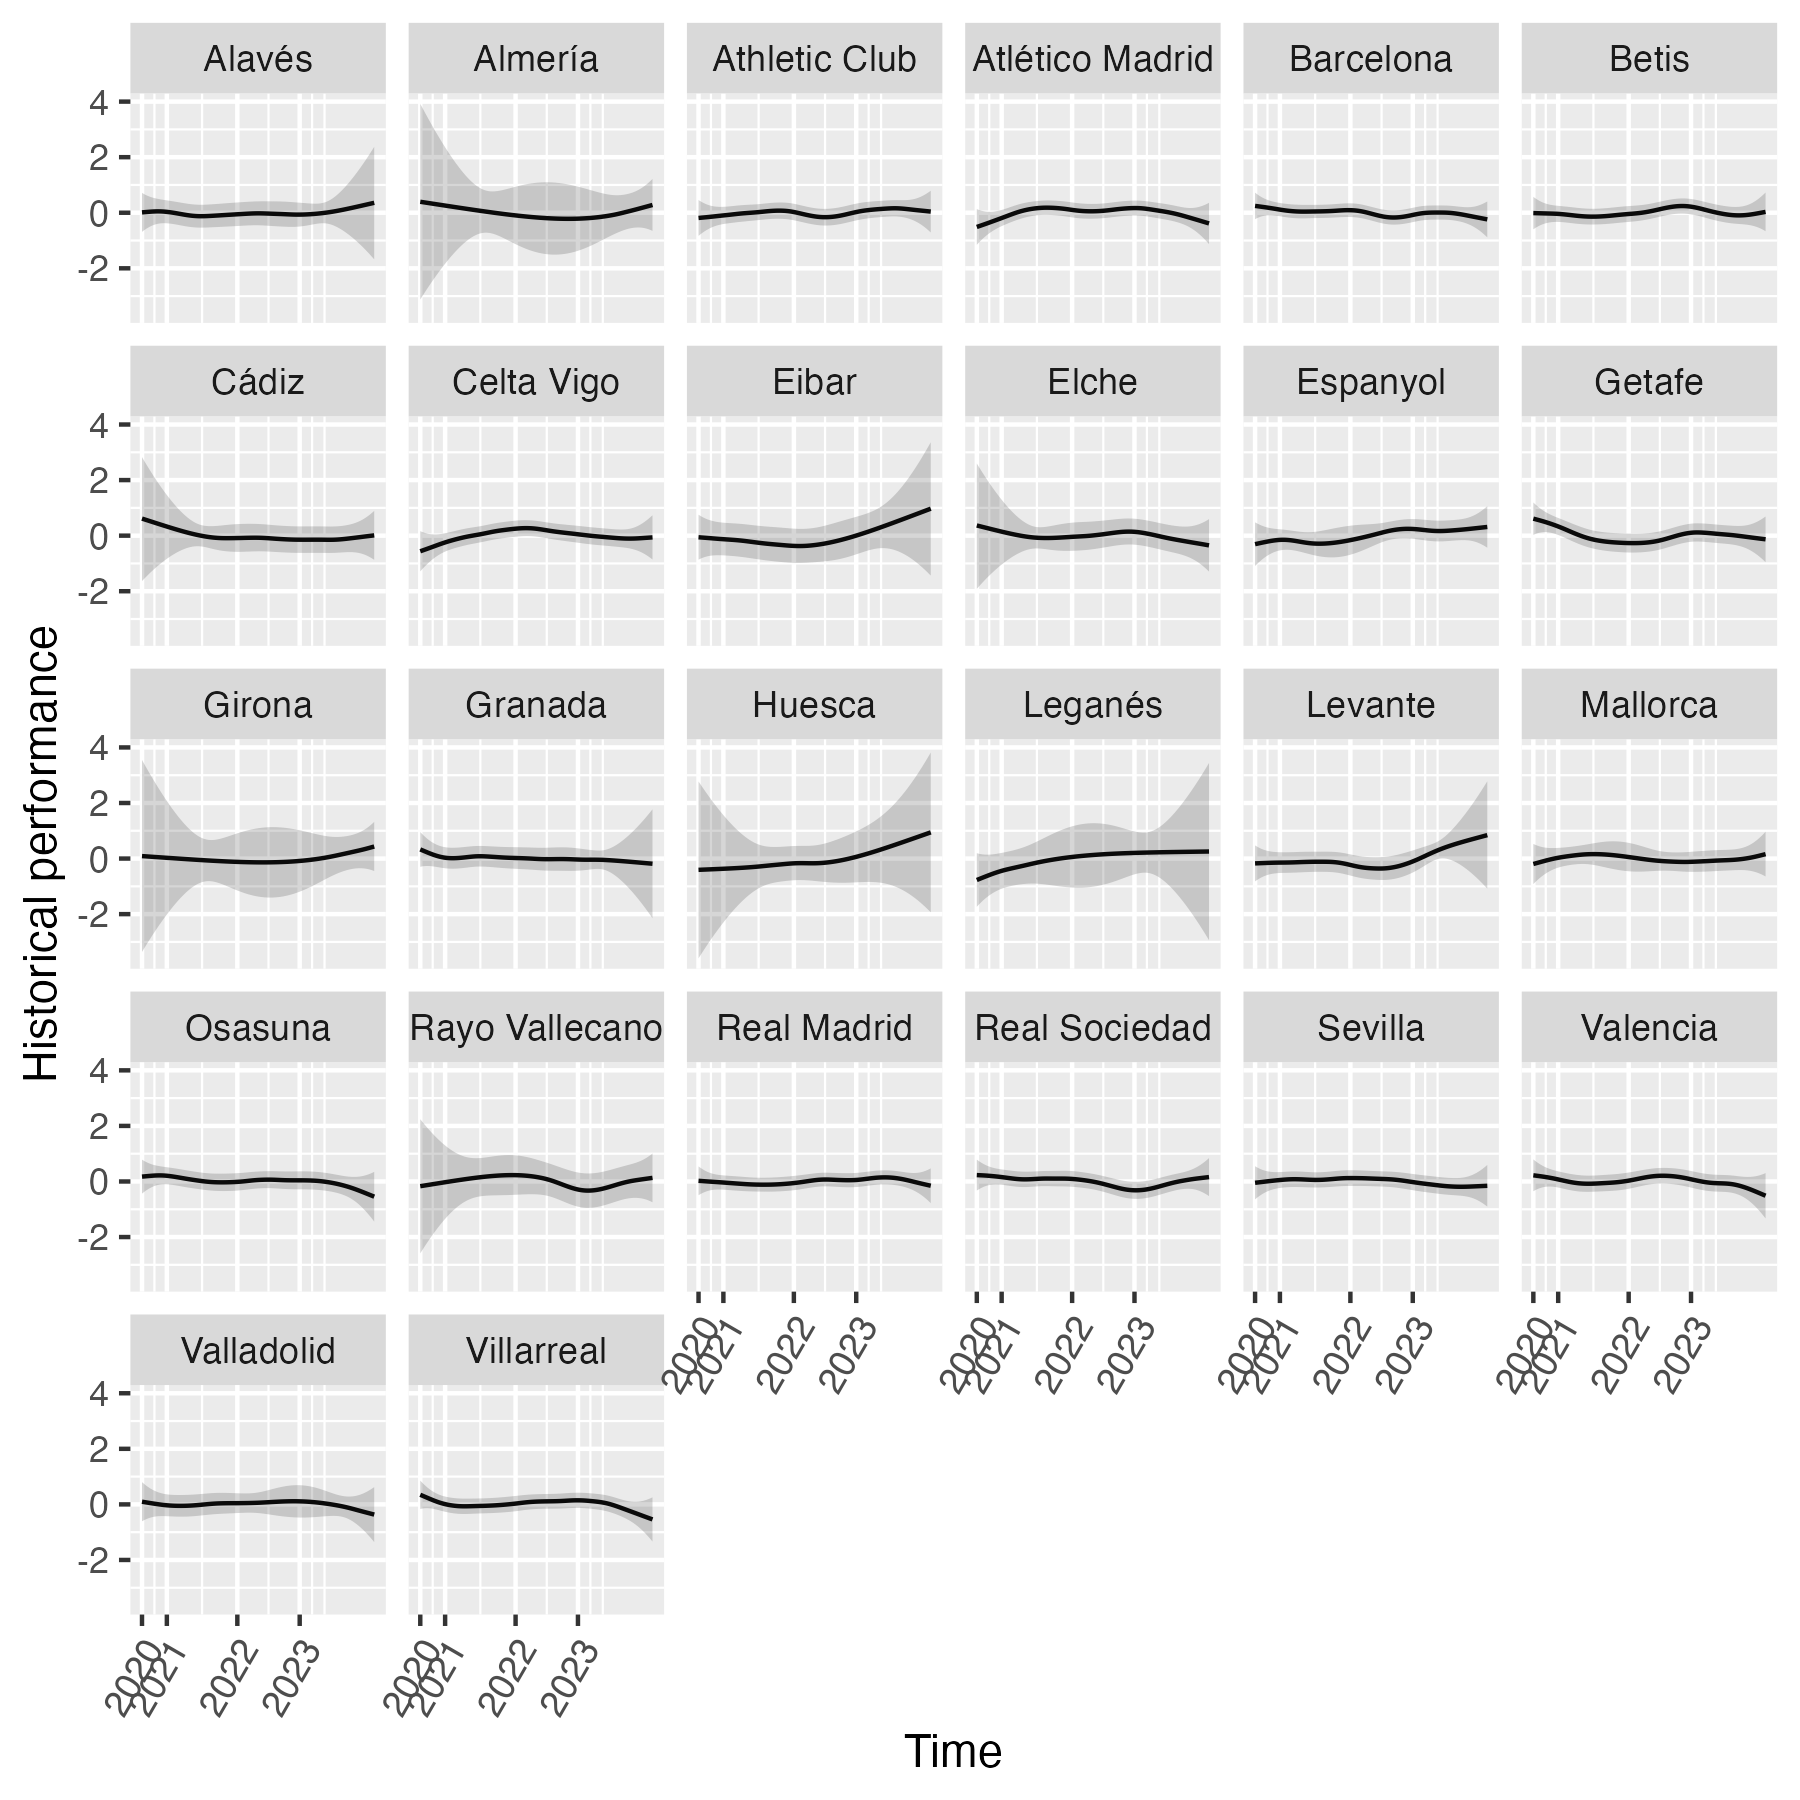
\includegraphics[width=25in]{LaligaTTplot}

Another are of Bayesian Hierarchical Modelling to consider is
overdispersion, a common feature in count data like goals scored in
football. Overdispersion occurs when variance of the observed data is
greater than what would be expected under a simple Poisson distribution,
thus we aim to capture extra variability that may not be accounted for
with other covariates. This is demonstrated in the code by
\texttt{f(num,model="iid")} which adds another random effect to the INLA
model, based on `num' which is the unique identifier of every row in the
data.

However after adding these variables individually and together, they did
not improve model fit by WAIC; adding the random walk time component
increased deviation, while adding the overdispersion parameter neither
improved or negatively impacts WAIC by a noticeable amount. We note the
very high in precision in the model hyperparameters for these added
random effects via the summary output, demonstrating the lack of
variability that is captured by these covariates. Thus we continue
without them.

\hypertarget{model-validation}{%
\subsection{Model Validation}\label{model-validation}}

In model validation we aim to compare the effectiveness of the more
complex `optimised' model, based off WAIC, and the baseline model. This
is executed using all the prior seasons data, with observed data up
until halfway through the 2021/22 season. We then simulate the remainder
of the 2021/22 seasons for each league, and compare with the observed
results of the final league positions for each team. The mean square
error of the optimised and baseline model are compared, and we proceed
to the 2022/23 modelling based on which model has lower MSE. Consider
the case of the Premier League model validation, the table below shows
the predictive performance of the

\begin{table}[!h]

\caption{\label{tab:unnamed-chunk-5}Comparing Baseline and Optimised models Performance vs Obesrved}
\centering
\resizebox{\linewidth}{!}{
\begin{tabular}[t]{l|r|r|r|r|r}
\hline
Team & Observed\_Points & Baseline\_Points & Baseline\_Difference & Optimized\_Points & Optimized\_Difference\\
\hline
Arsenal & 69 & 56 & 13 & 56 & 13\\
\hline
Aston Villa & 45 & 61 & 16 & 47 & 2\\
\hline
Brentford & 46 & 35 & 11 & 37 & 9\\
\hline
Brighton & 51 & 36 & 15 & 44 & 7\\
\hline
Burnley & 35 & 33 & 2 & 35 & 0\\
\hline
Chelsea & 74 & 67 & 7 & 61 & 13\\
\hline
Crystal Palace & 48 & 57 & 9 & 42 & 6\\
\hline
Everton & 39 & 37 & 2 & 39 & 0\\
\hline
Leeds United & 38 & 44 & 6 & 36 & 2\\
\hline
Leicester City & 52 & 51 & 1 & 47 & 5\\
\hline
Liverpool & 92 & 65 & 27 & 68 & 24\\
\hline
Manchester City & 93 & 86 & 7 & 74 & 19\\
\hline
Manchester Utd & 58 & 60 & 2 & 56 & 2\\
\hline
Newcastle Utd & 49 & 35 & 14 & 35 & 14\\
\hline
Norwich City & 22 & 34 & 12 & 31 & 9\\
\hline
Southampton & 40 & 41 & 1 & 42 & 2\\
\hline
Tottenham & 71 & 61 & 10 & 56 & 15\\
\hline
Watford & 23 & 32 & 9 & 28 & 5\\
\hline
West Ham & 56 & 62 & 6 & 54 & 2\\
\hline
Wolves & 51 & 56 & 5 & 51 & 0\\
\hline
\end{tabular}}
\end{table}

Using the figures above we are able to calculated the mean squared error
for the baseline model and optimised models respectively; 115.55, 100.65
thus demonstrating we have achieved better performance using the
optimised formula in the log linear model for the scoring parameters.
The improved performance is consistent with results of Bundesliga, Serie
A, and La Liga, all of which had lower MSE than their baseline models.
However in the case of Ligue 1, as the baseline model achieves lower
MSE. This may be due to the reduce number of data points used in
modelling. In the 2019/20 seasont the COVID-19 Pandemic resulted in the
distruption of football scheduling in the domestic leagues, and while
the other four returned to action, Ligue 1 ended halfway through. Thus
when modelling using data from 2019-2023, there are missing observations
that were removed for the French league. This means that the baseline
model, which is stronger at identifying variability in team attack and
defence random effects, may better fit the league with fewer data
available, since the otimised model may overfit the data.

We next model the 2022/23 seasons using the optimised log linear models
for the Premier League, Bundesliga, Serie A, and La liga, whilst using
the baseline model for Ligue 1.

\hypertarget{final-predictions}{%
\section{Final Predictions}\label{final-predictions}}

Now that we have final models to predict performances in the European
domestic leagues, we return to the original questions; How will the
teams perform in the 2022/2023 season? How will the results fair with
the removal of the Super League Teams?

\hypertarget{predicting-with-super-league-teams-included}{%
\subsubsection{Predicting with Super League Teams
Included}\label{predicting-with-super-league-teams-included}}

After modelling the 2022/23 seasons with the proposed `founding' members
of the super league and the teams likely to join, the league positions
are as follows: We notice that (summarise table here)

\begin{table}[!h]
\centering
\begin{tabular}{r|l|l|l|l|l}
\hline
League Position & Team (Premier League) & Team (La Liga) & Team (Serie A) & Team (Ligue 1) & Team (Bundesliga)\\
\hline
1 & Arsenal & Barcelona & Napoli & Paris S-G & Bayern Munich\\
\hline
2 & Manchester City & Real Madrid & Inter & Lens & Dortmund\\
\hline
3 & Manchester Utd & Real Sociedad & Juventus & Marseille & Union Berlin\\
\hline
4 & Newcastle Utd & Atlético Madrid & Milan & Monaco & Eint Frankfurt\\
\hline
5 & Tottenham & Betis & Roma & Lille & Freiburg\\
\hline
6 & Brentford & Rayo Vallecano & Lazio & Lorient & RB Leipzig\\
\hline
7 & Brighton & Athletic Club & Atalanta & Nice & Wolfsburg\\
\hline
8 & Fulham & Mallorca & Bologna & Rennes & M'Gladbach\\
\hline
9 & Liverpool & Villarreal & Torino & Reims & Köln\\
\hline
10 & Aston Villa & Osasuna & Udinese & Toulouse & Mainz 05\\
\hline
11 & Nott'ham Forest & Girona & Monza & Clermont Foot & Leverkusen\\
\hline
12 & Chelsea & Sevilla & Empoli & Lyon & Werder Bremen\\
\hline
13 & Leeds United & Celta Vigo & Lecce & Nantes & Augsburg\\
\hline
14 & Crystal Palace & Espanyol & Fiorentina & Montpellier & Bochum\\
\hline
15 & Leicester City & Valladolid & Sassuolo & Troyes & Hertha BSC\\
\hline
16 & Bournemouth & Almería & Salernitana & Ajaccio & Hoffenheim\\
\hline
17 & Everton & Cádiz & Spezia & Auxerre & Stuttgart\\
\hline
18 & Wolves & Getafe & Hellas Verona & Brest & Schalke 04\\
\hline
19 & West Ham & Valencia & Sampdoria & Strasbourg & NA\\
\hline
20 & Southampton & Elche & Cremonese & Angers & NA\\
\hline
\end{tabular}
\end{table}

\hypertarget{predicting-without-super-league-teams}{%
\subsubsection{Predicting Without Super League
Teams}\label{predicting-without-super-league-teams}}

After modelling the 2022/23 seasons without the proposed `founding'
members of the super league and the teams likely to join, the league
positions are as follows: We notice that (summarise table here)

\begin{table}[!h]
\centering
\begin{tabular}{r|l|l|l|l|l}
\hline
League Position & Team (Premier League) & Team (La Liga) & Team (Serie A) & Team (Ligue 1) & Team (Bundesliga)\\
\hline
1 & Newcastle Utd & Real Sociedad & Atalanta & Marseille & Eint Frankfurt\\
\hline
2 & Fulham & Betis & Bologna & Lens & Freiburg\\
\hline
3 & Brighton & Athletic Club & Cremonese & Lille & Union Berlin\\
\hline
4 & Aston Villa & Osasuna & Empoli & Lorient & RB Leipzig\\
\hline
5 & Brentford & Rayo Vallecano & Fiorentina & Monaco & Wolfsburg\\
\hline
6 & Crystal Palace & Girona & Hellas Verona & Nice & Mainz 05\\
\hline
7 & Nott'ham Forest & Mallorca & Lazio & Rennes & Leverkusen\\
\hline
8 & West Ham & Sevilla & Lecce & Reims & M'Gladbach\\
\hline
9 & Wolves & Villarreal & Monza & Toulouse & Werder Bremen\\
\hline
10 & Everton & Celta Vigo & Napoli & Clermont Foot & Köln\\
\hline
11 & Leicester City & Valladolid & Roma & Lyon & Bochum\\
\hline
12 & Leeds United & Espanyol & Salernitana & Nantes & Hertha BSC\\
\hline
13 & Bournemouth & Getafe & Sampdoria & Montpellier & Augsburg\\
\hline
14 & Southampton & Almería & Sassuolo & Ajaccio & Hoffenheim\\
\hline
15 & NA & Cádiz & Spezia & Troyes & Stuttgart\\
\hline
16 & NA & Valencia & Torino & Auxerre & Schalke 04\\
\hline
17 & NA & Elche & Udinese & Brest & NA\\
\hline
18 & NA & NA & NA & Strasbourg & NA\\
\hline
19 & NA & NA & NA & Angers & NA\\
\hline
20 & NA & NA & NA & NA & NA\\
\hline
\end{tabular}
\end{table}

\hypertarget{discussion}{%
\section{Discussion:}\label{discussion}}

\hypertarget{conclusions}{%
\subsection{Conclusions}\label{conclusions}}

\begin{itemize}
\tightlist
\item
  talk about what we foud in our results compare the Withoutsuperleague
  to withoutsuperleague preditions,
\item
  what are the supposed effect of these predictions? the significance?
\end{itemize}

\hypertarget{limitations}{%
\subsection{Limitations}\label{limitations}}

\begin{itemize}
\item
  A common probablem of the Bayesian Hierarchical model is overshrinkage
  where extreme outcomes, like a team scoring 8 goals, are instead
  pulled towards the grand mean. We notice this in the use of
\item
  Can improve performance using more data
\item
  Lack of Covariates
\end{itemize}

\hypertarget{future-work}{%
\subsection{Future Work}\label{future-work}}

\begin{itemize}
\item
  3 Tier Hierarchical Model
\item
  Machine Learning Techniques?
\item
  add more complex covariates ? player specific level perhaps?
\end{itemize}

etc.

\hypertarget{references-still-draft}{%
\section{References: (still draft)}\label{references-still-draft}}

BBC. (2021, April 20). European Super League offends principles of
competition - Boris Johnson. BBC News.
\url{https://www.bbc.co.uk/news/uk-56822592}

La Liga (December 15 2022). La Liga Newsletter: The Super League Would
be the end of a 100 Year Long Football Tradition. Accessed from:
\url{https://newsletter.laliga.es/global-futbol/a-kpmg-report-reveals-that-laliga-would-lose-55-of-its-revenues-with-the-creation-of-a-separatist-european-super-league}

{[}\url{https://www.statista.com/statistics/1230111/european-super-league-sponsorship-revenue/\#}:\textasciitilde:text=Early\%20reports\%20suggested\%20that\%20media,euros\%20annually\%20from\%20these\%20deals{]}

Reep, C., Pollard, R., \& Benjamin, B. (1971). Skill and Chance in Ball
Games. Journal of the Royal Statistical Society. Series A (General),
134(4), 623--629. \url{https://doi.org/10.2307/2343657}

Maher, M. J. (1982). Modelling association football scores. Statistica
Neerlandica, 36(3), 109-118.

Hvattum, L. M., \& Arntzen, H. (2010). Using ELO ratings for match
result prediction in association football. International Journal of
forecasting, 26(3), 460-470.

Rue, H., \& Salvesen, Ø. (2000). Prediction and Retrospective Analysis
of Soccer Matches in a League. Journal of the Royal Statistical Society.
Series D (The Statistician), 49(3), 399--418.
\url{http://www.jstor.org/stable/2681065}

Godin, F., Zuallaert, J., Vandersmissen, B., De Neve, W., \& Van de
Walle, R. (2014, June). Beating the bookmakers: leveraging statistics
and Twitter microposts for predicting soccer results. In KDD Workshop on
large-scale sports analytics (pp.~2-14). New York, NY, USA: ACM.

Baio, Gianluca \& Blangiardo, Marta. (2010). Bayesian hierarchical model
for the prediction of football results. Journal of Applied Statistics.
37. 253-264. 10.1080/02664760802684177.

Tsokos, Alkeos \& Kosmidis, Ioannis \& Baio, Gianluca \& Cucuringu,
Mihai \& Whitaker, Gavin \& Király, Franz. (2019). Modeling outcomes of
soccer matches. Machine Learning. 108. 10.1007/s10994-018-5741-1.
Hubáček, O., Šourek, G., \& Železný, F. (2019). Learning to predict
soccer results from relational data with gradient boosted trees. Machine
Learning, 108, 29-47.

Santos-Fernandez, E., Wu, P., \& Mengersen, K. L. (2019). Bayesian
statistics meets sports: a comprehensive review. Journal of Quantitative
Analysis in Sports, 15(4), 289-312.

Schauberger, G., \& Groll, A. (2018). Predicting matches in
international football tournaments with random forests. Statistical
Modelling, 18(5-6), 460-

Hilbe, J. M., De Souza, R. S., \& Ishida, E. E. (2017). Bayesian models
for astrophysical data: using R, JAGS, Python, and Stan. Cambridge
University Press.

H. Rue, S. Martino, and N. Chopin. Approximate Bayesian inference for
latent Gaussian models using integrated nested Laplace approximations
(with discussion). Journal of the Royal Statistical Society, Series B,
71(2):319\{392, 2009.

Karlis, D., \& Ntzoufras, I. (2003). Analysis of sports data by using
bivariate Poisson models. Journal of the Royal Statistical Society:
Series D (The Statistician), 52(3), 381-393.

Müller K, Wickham H (2022). tibble: Simple Data Frames. R package
version 3.1.8, \url{https://CRAN.R-project.org/package=tibble}.

Wickham H, Averick M, Bryan J, Chang W, McGowan LD, François R,
Grolemund G, Hayes A, Henry L, Hester J, Kuhn M, Pedersen TL, Miller E,
Bache SM, Müller K, Ooms J, Robinson D, Seidel DP, Spinu V, Takahashi K,
Vaughan D, Wilke C, Woo K, Yutani H (2019). ``Welcome to the
tidyverse.'' Journal of Open Source Software, 4(43), 1686.
\url{https://doi.org/10.21105/joss.01686}.

Wickham H, François R, Henry L, Müller K, Vaughan D (2023). \emph{dplyr:
A Grammar of Data Manipulation}. R package version 1.1.0,
\url{https://CRAN.R-project.org/package=dplyr}.

H. Rue, S. Martino, and N. Chopin. Approximate Bayesian inference for
latent Gaussian models using integrated nested Laplace approximations
(with discussion). Journal of the Royal Statistical Society, Series B,
71(2):319, p392, 2009.

Gelman, A., Hwang, J. \& Vehtari, A. Understanding predictive
information criteria for Bayesian models. Stat Comput 24, 997--1016
(2014). \url{https://doi.org/10.1007/s11222-013-9416-2}

\end{document}
